\documentclass[fontsize=12pt, paper=a4, headinclude, twoside=false, parskip=half+, pagesize=auto, numbers=noenddot, plainheadsepline, open=right, toc=listof, toc=bibliography]{scrreprt}

% Abstand über Chapter Überschrift verringern
\renewcommand*{\chapterheadstartvskip}{\vspace*{-10pt}}
% PDF-Kompression
\pdfminorversion=5
\pdfobjcompresslevel=1
% Allgemeines
\usepackage[automark]{scrlayer-scrpage} % Kopf- und Fußzeilen
\usepackage{amsmath} % Mathesachen
\newtheorem{definition}{Definition}
\usepackage[T1]{fontenc} % Ligaturen, richtige Umlaute im PDF
\usepackage[utf8]{inputenc}% UTF8-Kodierung für Umlaute usw
\usepackage{hyphenat}
% Schriften
%\usepackage{mathpazo} % Palatino für Mathemodus
%\usepackage{tgpagella} % auch sehr schöne Schriften
\usepackage{lmodern}
\usepackage{caption}
%Courier 
% \usepackage{mathptmx}
% \usepackage[scaled=.90]{helvet}
% \usepackage{courier}
\usepackage{setspace} % Zeilenabstand
\usepackage{adjustbox}
\usepackage{hhline}
\usepackage{tikz}
%\usepackage{gb4e}
\usetikzlibrary{fit, positioning, shapes.geometric, decorations.pathreplacing,positioning, arrows.meta}

\onehalfspacing % 1,5 Zeilen
% Kein Seitenumbruch bei neuem Chapter
\usepackage{etoolbox}
\makeatletter
\patchcmd{\chapter}{\if@openright\cleardoublepage\else\clearpage\fi}{}{}{}
\makeatother
% Gliederungstiefe
\setcounter{tocdepth}{3}
\setcounter{secnumdepth}{3} 
% Schriften-Größen
\setkomafont{chapter}{\Huge\sffamily} % Überschrift der Ebene
\setkomafont{section}{\Large\sffamily}
\setkomafont{subsection}{\large\sffamily}
\setkomafont{subsubsection}{\large\sffamily}
\setkomafont{chapterentry}{\large\sffamily} % Überschrift der Ebene in Inhaltsverzeichnis
\setkomafont{descriptionlabel}{\bfseries\sffamily} % für description Umgebungen
\setkomafont{captionlabel}{\small\sffamily}
\setkomafont{caption}{\small\sffamily}
%\setkomafont{captionof}{\small\sffamily}
\setkomafont{footnote}{\sffamily}
% Sprache: Deutsch, Englisch als default
\usepackage[german, english]{babel} % Silbentrennung
\usepackage[babel]{csquotes} % Anführungszeichen mit enquote
% Tabellen
\usepackage{multirow} % Tabellen-Zellen über mehrere Zeilen
\usepackage{multicol} % mehre Spalten auf eine Seite
\usepackage{tabularx} % Für Tabellen mit vorgegeben Größen
\usepackage{longtable} % Tabellen über mehrere Seiten
\usepackage{array}
\usepackage{setspace}
\usepackage{threeparttable}
%  Bibliographie
%\usepackage{bibgerm} % Umlaute in BibTeX
%\usepackage{authordate1-4}
\usepackage{natbib}
\bibliographystyle{unsrtnat}
% Tabellen
\usepackage{multirow} % Tabellen-Zellen über mehrere Zeilen
\usepackage{multicol} % mehre Spalten auf eine Seite
\usepackage{booktabs} % Für Tabellen mit bottom, mid, toprule (schöner als hline)
\usepackage{tabularx} % Für Tabellen mit vorgegeben Größen
\usepackage{array}
\usepackage{float}
% Bilder
\usepackage{graphicx} % Bilder
\usepackage{color} % Farben
%\usepackage[usenames,dvipsnames]{xcolor}
\graphicspath{{images/}}
\DeclareGraphicsExtensions{.pdf,.png,.jpg} % bevorzuge pdf-Dateien
\usepackage{subfigure} % mehrere Abbildungen nebeneinander/übereinander
\newcommand{\subfigureautorefname}{\figurename} % um \autoref auch für subfigures benutzen
% Bildunterschrift
\setcapindent{0em} % kein Einrücken der Caption von Figures und Tabellen
\setcapwidth[c]{0.9\textwidth}
\setlength{\abovecaptionskip}{0.2cm} % Abstand der zwischen Bild- und Bildunterschrift
% Quellcode
\usepackage{listings} % für Formatierung in Quelltexten
\definecolor{grau}{gray}{0.45}
\lstset{
	extendedchars=true,
	basicstyle=\tiny\ttfamily,
	%basicstyle=\footnotesize\ttfamily,
	tabsize=2,
	keywordstyle=\textbf,
	commentstyle=\color{grau},
	stringstyle=\textit,
	numbers=left,
	numberstyle=\tiny,
	% für schönen Zeilenumbruch
	breakautoindent  = true,
	breakindent      = 2em,
	breaklines       = true,
	postbreak        = ,
	prebreak         = \raisebox{-.8ex}[0ex][0ex]{\Righttorque},
}
% linksbündige Fußnoten
\deffootnote{1.5em}{1em}{\makebox[1.5em][l]{\thefootnotemark}}
% PDF
\usepackage[english,pdfauthor={Julia Kreutzer},pdfauthor={Julia Kreutzer},pdftitle={--}, breaklinks=true,pdfpagelabels,plainpages=false]{hyperref}
\usepackage[final]{microtype} % mikrotypographische Optimierungen
\usepackage{url}
\usepackage{pdflscape} % einzelne Seiten drehen können
\usepackage[all]{hypcap} % Beim Klicken auf Links zum Bild und nicht zu Caption gehen

\usepackage{epstopdf} %eps to pdf 
\usepackage{pdfpages}


\usepackage{chngcntr}
\usepackage{gb4e}

\noautomath
 
\counterwithout{figure}{chapter}
\counterwithout{table}{chapter}
\counterwithout{equation}{chapter}

\typearea{14} % typearea am Schluss berechnen lassen, damit die Einstellungen oben berücksichtigt werden
% für autoref von Gleichungen in itemize-Umgebungen
\makeatletter

%\newcommand{\saved@equation}{}
%\let\saved@equation\equation
%\def\equation{\@hyper@itemfalse\saved@equation}
%\makeatother 

% argmax als Befehl in Formeln
\DeclareMathOperator*{\argmax}{argmax}

% Eigene Befehle %%%%%%%%%%%%%%%%%%%%%%%%%%%%%%%%%%%%%%%%%%%%%%%%%5
% Matrix
\newcommand{\mat}[1]{
      {\textbf{#1}}
}
\newcommand{\todo}[1]{
      {\colorbox{red}{ TODO: #1 }}
}
\newcommand{\todotext}[1]{
      {\color{red} TODO: #1} \normalfont
}

\newcommand{\todoref}[1]{
	  {\colorbox{yellow}{ REFERENCE: #1 }}
}

\newcommand{\info}[1]{
      {\colorbox{green}{ (INFO: #1)}}
}
% Hinweis auf Programme in Datei
\newcommand{\datei}[1]{
      {\ttfamily{#1}}
}
\newcommand{\code}[1]{
      {\ttfamily{#1}}
}
% bild mit defnierter Breite einfügen
\newcommand{\bild}[4]{
  \begin{figure}[!hbt]
    \centering
      \vspace{1ex}
      \includegraphics[width=#2]{images/#1}
      \caption[#4]{\label{img.#1} #3}
    \vspace{1ex}
  \end{figure}
}
% bild auf eigener Seite
\newcommand{\bildp}[4]{
  \begin{figure}[p]
    \centering
      \vspace{1ex}
      \includegraphics[width=#2]{images/#1}
      \caption[#4]{\label{img.#1} #3}
    \vspace{1ex}
  \end{figure}
}
% bild mit eigener Breite
\newcommand{\bilda}[3]{
  \begin{figure}[!hbt]
    \centering
      \vspace{1ex}
      \includegraphics{images/#1}
      \caption[#3]{\label{img.#1} #2}
      \vspace{1ex}
  \end{figure}
}


% Bild todo
\newcommand{\bildt}[2]{
  \begin{figure}[!hbt]
    \begin{center}
      \vspace{2ex}
	      \includegraphics[width=6cm]{images/todobild}
      \caption{\label{#1} \todotext{#2}}
      \vspace{2ex}
    \end{center}
  \end{figure}
}

\newcommand{\ra}[1]{\renewcommand{\arraystretch}{#1}}

%\texttt{\newcommand\Chapter[2]{
%  \chapter[{\scshape#1}: {\itshape#2}]{\scshape#1\\\normalsize\itshape --#2}
%} % Importiere die Einstellungen aus der Präambel
% hier beginnt der eigentliche Inhalt
\begin{document}
\sffamily
\pagenumbering{Roman} % große Römische Seitenummerierung
\pagestyle{plain}
%\selectlanguage{english}

% Titelseite
\clearscrheadings\clearscrplain



\begin{center}

\begin{Huge}
\vspace{10mm}
\textbf{Identifying and Quantifying Aspectual Ambiguity with LMs}
\end{Huge}\\[5mm]
\textbf{\Large Reversing the NLP Pipeline}


\vspace{70mm}
\begin{large}
Bachelor Thesis\\
Date, Year\\
%\vspace{0.4cm}

\vspace{1 cm}
Samuel Innes\\
innes@cl.uni-heidelberg.de\\
\end{large}
\vspace{2cm}

\begin{Large}
Institut für Computerlinguistik\\ % remove either en or de
\vspace{3mm}
\end{Large}{\Large Ruprecht-Karls-Universität Heidelberg}\\ %remove either en or de
\vspace{2cm}

\begin{tabular}{ll}
\textbf{Supervisor} & Prof. Dr. Michael Herweg\\
\textbf{Reviewer} & Prof. Dr. Katja Markert\\
\end{tabular}
\end{center}

\clearpage


\pagestyle{useheadings} % normale Kopf- und Fußzeilen für den Rest

\chapter*{Abstract}\label{c.abstract}
Abstract in English

\clearpage
\chapter*{Zusammenfassung}\label{c.zusammenfassung}
\foreignlanguage{ngerman}{
Zusammenfasssung auf Deutsch
}

\clearpage
\tableofcontents
\clearpage
\listoffigures
\clearpage
\listoftables

% richtiger Inhalt
\clearpage
\pagenumbering{arabic} % ab jetzt die normale arabische Nummerierung
\chapter{Introduction}\label{c.introduction}
\section*{Motivation}
Despite being one of the most studied areas in linguistics, I COULDNT FIND ANY statistical approaches to aspect. 
\section*{Why aspect?}
One may justifiably beg the question why a “computational approach” to aspect (OR INDEED TO ANY PROBLEM IN THEORETICAL LINGUISTICS) is necessary or indeed useful: in an age of LLMs

The use of such a study comes down to the purpose of computational linguistics as an area of study. Computational linguistics has changed a lot since its conception in the mid 20th century, at some points being closer to linguistics and at others (arguably including right now) being closer to computer science. However the position of the field lying at the intersection between more well-established and well-defined areas of study has led to a fruitful exchange of ideas between the disciplines.\footnote{Just to name a few examples: formal languages, artificial neural networks and SOMETHING ELSE!!!!!!}

One reason is of course the contribution to the linguistic community: computational approaches to language have SPURRED ON LOTS OF PROGRESS (cf Chomsky!!!). A 

In the true nature of the interdisciplinarity of the field I wish to WORK AT BOTH AIMS IN PARALLEL and show how they complement each other.

Importance on engineering side:
\begin{itemize}
    \item{Zero-shot performance of ChatGPT comparable with BERT \citep{zhong2023chatgpt}}
    \item{I also experienced poor (?) performance with own experiments}
    \item{but fine-tuning lead to large improvements}
    \item UMR annotates aspect, and this can be used to extract habitual events or states, which are typical knowledge forms
\end{itemize}

The fact that fine-tuning can lead the model to 

Therefore the purpose of this study is two-fold: firstly to further explore the phenomenology of aspect using methods from computational linguistics such as neural embeddings, and secondly to look at how current state-of-the-art approaches deal with this phenomenon and investigate how this could be improved.


I wish to challenge Chomsky's assertion that large language models are "not a contribution to science"\footnote{https://www.youtube.com/watch?v=axuGfh4UR9Q WHAT TIME DOES HE SAY THIS???}

\section*{Main contributions}
\begin{itemize}
    \item First in-depth study using computational approaches to study the phenomenology of aspect 
    \item First probing of neural models applied to the task
    \item SOMETHING ELSE
\end{itemize}
\section*{Structure of this thesis}

\chapter{Aspectology: an introduction}\label{c.aspectology}
Many works on the area begin with the assertion that aspect is one of the most studied areas of linguistics \citep{Sasse2002RecentAI}, particularly Slavic linguistics (for reasons I will discuss later), and hence a thorough theoretical discussion of the linguistic phenomenon which does full justice to the work on the field is not possible within the constraints of this thesis. Nevertheless, in order to give an introduction to the fundamental elements of the following study and make a productive contribution to the area, I will touch on some of the main findings in the area of aspectology.
\section{A (short) phenomenology of aspect}
The Concise Oxford Dictionary of Linguistics \citep{matthews2014concise} defines aspect thus: 

\begin{quotation}
    [Aspect is a g]eneral term, originally of specialists in Slavic languages, for verbal categories that distinguish the status of events, etc. in relation to specific periods of time, as opposed to their simple location in the present, past, or future.
\end{quotation}

As noted here, one helpful distinction which must be made right away is that between \emph{aspect}, and another temporal phenomenon \emph{tense}. Many works recall Bernard Comrie's differentiation in his book \emph{Aspect} \citep{comrie1976aspect} between the deictic nature of \emph{tense} and the focus on the "internal temporal constituency of a situation" of \emph{aspect}. In other words: "tense\footnote{In many of the world's languages this is grammaticalised as past, present and future; in others such as English by some accounts \citep{jespersen2013essentials} it is a binary distinction such as past and non-past, whereas some languages such as Greenlandic (Kalaallisut) some linguists have even argued to be tenseless \citet{10.1093/jos/ffh029}. See also the contentious debate about Hopi time \citet{whorf-writings, hopitime}. } relates the time of the situation referred to to some other time, usually to the moment of speaking", and thus by relating the time of the situation to the time of the utterance it is deictic \citep{comrie1976aspect}. Aspect on the other hand gives a \emph{situation-internal} description of the events in that situation, such how they relate to each other temporally or how an individual event is temporally characterised. This introduces another important distinction: that between lexical and grammatical aspect.

\begin{figure}
    \begin{tikzpicture}
        \foreach \x/\z [count=\y] in {Time/yellow,Situation/orange,Event/red} {
            \draw[fill=\z] (0,{\y-4}) circle[radius={4-\y}];
            \node at (0,{-2*(4-\y)+1}) {\x};
        } 
    \end{tikzpicture}
    \hspace{2cm}
    \begin{tikzpicture}
        \node {Situation}[sibling distance = 3.5cm, level distance = 2cm]
        child [red] {node {Tense} 
            edge from parent [blue] node [left] {external}}
        child {node {Event} 
            child [red] {node {Grammatical aspect}
                edge from parent [blue] node [left] {external}}
            child [red] {node {Lexical aspect}
                edge from parent [blue] node [right] {internal}} 
            edge from parent [blue] node [right] {internal}};
    \end{tikzpicture}
    \caption{A set-theoretical representation of the relationship between time, situation and event \emph{(left)} along with the categorisation of the three temporal phenomena discussed \emph{(right)}.}
    \label{fig:TimeSitEvent}
\end{figure}

\subsection{Lexical vs grammatical aspect}
The polysemy of the term “aspect” in the linguistic community is unfortunate. In an area of language which seems to have surprisingly far-reaching interactions with other parts of linguistic systems these ambiguities are particularly unhelpful.\footnote{Among other things, aspect is also intertwined with case, mood and voice \citep{franks2005slavic, Kiparsky2004PartitiveCA}.}
As already mentioned, aspect\footnote{Boogaart uses the term \emph{aspectuality} to remove the aforementioned ambiguity \citep{Boogaart+2004+1165+1180}. However, I will stick with the term \emph{aspect} due to its prevalence in the literature, further specifying where necessary.} is a term often used to refer to both lexical and grammatical aspect. Lexical aspect (also referred to as \emph{Aktionsart, situation aspect} or \emph{inner aspect}) is the inherent property of a verb or verb phrase which “characterizes the temporal profile of event descriptions” \citep{10.1093/oxfordhb/9780199601264.013.25}. For example, to “crack open an egg” is inherently a short event describing the change of one state (the egg being whole) to another (the egg being cracked). Grammatical aspect (or \emph{viewpoint aspect, outer aspect}), on the other hand, describes the “internal temporal constituency” \citep{comrie1976aspect} XCHANGE THIS!! of an event, such as its habituality or ongoing nature and can be seen more as an external lens imposed on a verbal phrase. In English, one example of this lens is the progressive, which is formed by the verb \emph{be} + gerund, as in the phrase “Sue was running”. 

Figure \ref{fig:TimeSitEvent} shows a taxonomy of tense, and grammatical and lexical aspect. An event is an atomic or 

Here each situation is a union of events ($\mathbf{situations} = \mathcal{P}(\mathbf{events}) \setminus \emptyset$) and the 

Situations are anchored in time. 

The concrete linguistic realisation of these categories is very often unclear or non-existent and exhibits a relatively wide variety of encodings throughout the world’s languages \citep{Dahl1985TenseAA}. It therefore proves tricky to uphold this distinction in empirical studies "in the real world". This has led some to question to what extent this distinction makes sense \citep{Sasse2002RecentAI}. Those who question the contrast between these two semantic dimensions, described as unidimensionalists in \citet{Sasse2002RecentAI}, claim that aspectual distinctions in both dimensions can be reduced to a common set of semantic primitives, which can be applied to all levels of analysis, i.e. the boundedness of lexical aspect is the same as the boundedness which marks the distinction between the perfective and imperfective parameters. 

I have chosen to introduce this distinction in order to WHAT

WHICH MODEL WOULD I LIKE TO USE IN THE END??

Nevertheless the theoretical differentiation of these two interrelated subdomains is an important one to make, and each describes a variety of concepts which will be useful later.

\subsection{Lexical aspect}
\subsection*{Telicity}
A fundamental distinction of lexical aspect is that of telicity (from Ancient Greek \emph{télos} meaning “end”). Telicity describes whether an event has an inherent goal or end-point after which the event can be regarded as completed: for example "go climbing" would be atelic whereas "climb the mountain" is telic (since it involves the agent reaching the summit of a mountain). A classic test for telicity\footnote{Though \citet{XiaoMcenery+2006+1+21} note that this test is flawed and propose an alternative test scheme.} is whether the verb phrase admits a completing adverb such as "in an hour" and does not admit a durative adverb such as "for an hour" \citep{Krifka1998TheOO}.

Dahl misleadingly defines telicity as "involv[ing] the presence of a boundary or the attainment of a specific result-state" \citep{DAHL2015210}, which, however can lead to confusion with the term \emph{(un)boundedness}.
\subsection*{Boundedness}
(Un)boundedness refers to the existance (or lack of) a \emph{temporal} boundary marking the end of an action. Boundedness must be distinguished from telicity\footnote{\citet{friedrich-etal-2023-kind} seem to mistakenly conflate the two, stating that "[t]elicity is also sometimes referred to as boundedness (e.g., by Loáiciga and Grisot, 2016)" referring to the 2016 paper \citet{loaiciga-grisot-2016-predicting}, which, however, clearly distinguishes between the two notions.} in order to avoid the so-called 'Imperfective Paradox' highlighted by \citet{Linguistics2005DowtyD1}, here verbalised by \citet{zucchi}:

\begin{quotation}
    How is it possible that a statement of the form \emph{x was F-ing} is true and yet there
    is no time at which \emph{x was F-ed} is true?
\end{quotation}
More concretely, it asks the question why (\ref{para1}) entails (\ref{para2}) but (\ref{para3}) doesn't entail (\ref{para4}) in the examples below:
\begin{exe}
    \ex The man was running.
    \label{para1}
    \ex The man ran.
    \label{para2}
    \ex The man was building a house.
    \label{para3}
    \ex The man built a house.
    \label{para4}
\end{exe}
\citet{6608d9d0-a477-39af-8491-2172df5ae612} shows that this apparent "paradox" can be resolved by distinguishing between these two concepts of telicity and boundedness,\footnote{By definition of telicity as whether an even has an inherent end-point, and boundedness as whether it has a temporal boundary (separate from its intended end-point) we can distinguish between whether an event has reached its termination or whether it was ended before reaching this end-point. Therefore while it is the case that the both (\ref{para1}) and (\ref{para2}) are bounded, only (\ref{para3}) and (\ref{para4}) contain telic events, and it seems to be the case that the progressive's focus on temporal boundary nullifies the end-point inherent in the verb phrase "build a house". This serves as an interesting example of the interaction between grammatical and lexical aspect.} and this further serves to show the dangers of misuse of terminology. Table \ref{table:runreftime} visualises the relationship between the reference time (temporal boundaries) and the run-time (the inherent "time schema" of the verb phrase). This allows for a clearer definition of boundedness, namely whether the right-hand side of the run-time boundary lies within the reference time or not (IS THIS TRUE?).


\begin{table}
    \centering
    \begin{tabular}{|m{0.3\linewidth} |m{0.3\linewidth}| m{0.2\linewidth}| m{0.2\linewidth}|} \hline
        Sentence & Representation & Telicity & Boundedness \\ \hline \hline
        The man was running. &         \begin{tikzpicture}[scale=0.8]
            \draw [use as bounding box, draw=none] (0cm,-1.2cm) rectangle (6cm,1.2cm);
            % draw horizontal line   
            \draw[ultra thick, ->] (0,0) -- (5cm,0);
            %\node at (0,2) {The man};
            % draw node
            \draw[ultra thick] (4,0) node[below=3pt,thick] {} node[above=3pt] {};
            \draw[ultra thick] (6,0) node[below=3pt,thick] {} node[above=3pt] {};
            \draw[ultra thick] (8,0) node[below=3pt, thick] {} node[above=3pt] {};
                         \draw[ultra thick] (10,0) node[below=3pt] {} node[above=3pt] {};
            
            \draw [black, ultra thick ,decorate,decoration={brace,amplitude=5pt}] (2,0.2)  -- (3,0.2) 
                   node [black,midway,above=4pt,xshift=-2pt] {\footnotesize Reference time};
            
            
            \draw [ black, ultra thick,decorate,decoration={brace,amplitude=5pt, mirror}] (1,-0.2) -- (4,-0.2)
                   node [black,midway,below=4pt,xshift=8pt] {\footnotesize Run-time};


            % draw vertical lines
            \foreach \x in {1,2,3,4}
            \draw (\x cm,3pt) -- (\x cm,-3pt);
            \end{tikzpicture} & atelic & unbounded \\ \hline
            The man ran. &     \begin{tikzpicture}[scale=0.8]
                % draw horizontal line   
                \draw [use as bounding box, draw=none] (0cm,-1.2cm) rectangle (6cm,1.2cm);
                \draw[ultra thick, ->] (0,0) -- (5cm,0);
        
                %\draw[node at (0,2) {The man was building a house.}];
                %\node at (0,2) {The man};
        
                % draw node
                \draw[ultra thick] (4,0) node[below=3pt,thick] {} node[above=3pt] {};
                \draw[ultra thick] (6,0) node[below=3pt,thick] {} node[above=3pt] {};
                \draw[ultra thick] (8,0) node[below=3pt, thick] {} node[above=3pt] {};
                             \draw[ultra thick] (10,0) node[below=3pt] {} node[above=3pt] {};
                
                \draw [black, ultra thick ,decorate,decoration={brace,amplitude=5pt}] (1,0.2)  -- (4,0.2) 
                       node [black,midway,above=4pt,xshift=-2pt] {\footnotesize Reference time};
                
                
                \draw [ black, ultra thick,decorate,decoration={brace,amplitude=5pt, mirror}] (2,-0.2) -- (3.5,-0.2)
                       node [black,midway,below=4pt,xshift=8pt] {\footnotesize Run-time};

                            % draw vertical lines
            \foreach \x in {1,2,3.5,4}
            \draw (\x cm,3pt) -- (\x cm,-3pt);
                \end{tikzpicture} & atelic & bounded \\ \hline
            The man was building a house. & \begin{tikzpicture}[scale=0.8]
                \draw [use as bounding box, draw=none] (0cm,-1.6cm) rectangle (6cm,1.2cm);
                % draw horizontal line   
                \draw[ultra thick, ->] (0,0) -- (5cm,0);
                %\node at (0,2) {The man};
                % draw node
                \draw[ultra thick] (4,0) node[below=3pt,thick] {} node[above=3pt] {};
                \draw[ultra thick] (6,0) node[below=3pt,thick] {} node[above=3pt] {};
                \draw[ultra thick] (8,0) node[below=3pt, thick] {} node[above=3pt] {};
                             \draw[ultra thick] (10,0) node[below=3pt] {} node[above=3pt] {};
                
                \draw [black, ultra thick ,decorate,decoration={brace,amplitude=5pt}] (2,0.2)  -- (3,0.2) 
                       node [black,midway,above=4pt,xshift=-2pt] {\footnotesize Reference time};
                
                
                \draw [ black, ultra thick,decorate,decoration={brace,amplitude=5pt, mirror}] (1,-0.2) -- (4,-0.2)
                       node [black,midway,below=4pt,xshift=8pt] {\footnotesize Run-time};



                            % draw vertical lines
            \foreach \x in {1,2,3,4}
            \draw (\x cm,3pt) -- (\x cm,-3pt);

            \node[align=center] at (4,-1.35) {\footnotesize Goal};
            \draw [thick] (4,-1.2) -- (4,-0.15);
                \end{tikzpicture} & telic & unbounded \\ \hline
            The man built a house. & \begin{tikzpicture}[scale=0.8]
                % draw horizontal line   
                \draw [use as bounding box, draw=none] (0cm,-1.6cm) rectangle (6cm,1.2cm);
                \draw[ultra thick, ->] (0,0) -- (5cm,0);
        
                %\draw[node at (0,2) {The man was building a house.}];
                %\node at (0,2) {The man};
        
                % draw node
                \draw[ultra thick] (4,0) node[below=3pt,thick] {} node[above=3pt] {};
                \draw[ultra thick] (6,0) node[below=3pt,thick] {} node[above=3pt] {};
                \draw[ultra thick] (8,0) node[below=3pt, thick] {} node[above=3pt] {};
                             \draw[ultra thick] (10,0) node[below=3pt] {} node[above=3pt] {};
                
                \draw [black, ultra thick ,decorate,decoration={brace,amplitude=5pt}] (1,0.2)  -- (4,0.2) 
                       node [black,midway,above=4pt,xshift=-2pt] {\footnotesize Reference time};
                
                
                \draw [ black, ultra thick,decorate,decoration={brace,amplitude=5pt, mirror}] (1.5,-0.3) -- (3.5,-0.3)
                       node [black,midway,below=4pt,xshift=2pt] {\footnotesize Run-time};

                            % draw vertical lines
            \foreach \x in {1,1.5,3.5,4}
            \draw (\x cm,3pt) -- (\x cm,-3pt);

            \node[align=center] at (4,-1.35) {\footnotesize Goal};
            \draw [thick] (4,-1.2) -- (3.5,-0.15);
                \end{tikzpicture} & telic & bounded \\ \hline
    \end{tabular}
    \caption{Representation of (\ref{para1}),(\ref{para2}),(\ref{para3}) and (\ref{para4}) with regards to the reference time referred to by the utterance and inherent run-time of the event. Concept adapted from \citet{10.1093/oxfordhb/9780199601264.013.25}.}
\end{table}
\label{table:runreftime}

\subsection*{Stativity}
Another parameter of lexical aspect I would like to discuss is stativity, which describes a state of being such as "know", "love" or "be", rather than an action \citep{binnick1991time}. A classic test for stativity in English is non-admittance of the progressive or the imperative \citep{McINTOSH+1975+35+42}.\footnote{Interestingly, however, \citet{Granath_Wherrity_2013} find that, assuming a functional-semantic definition if stativity, the usage of stative verbs with the progressive is much higher in spoken language, than in written language.} Consider the following examples:
\begin{exe}
    \ex[]{She resembles her grandmother.}
    \ex[*]{She is resembling her grandmother.}
\end{exe}
\subsection*{Durativity}
Durativity denotes whether an event takes time (i.e. has duration) or happens in an instant, and this can be checked in English by the compatibility of durative adverbs such as \emph{for an hour} \citep{102998}. For example:
\begin{exe}
    \ex[]{Andrea was painting a picture for an hour.}
    \ex[*]{Andrea was reaching the summit for an hour.}
\end{exe}
\subsubsection{Some attempts at event classification}
\subsection*{\citet{vendler57}}
It was the seminal work \emph{Verbs and Times} \citep{vendler57} of philosopher Zeno Vender which initiated the discussion on inner aspect in the linguistic tradition.\footnote{A similar classification was also developed independently by Anthony Kenny in \emph{Action, Emotion and Will} \citep{Kenny1963-KENAEA}, however combining Achievement and Accomplishment into one single class \citep{19c36731-bdec-362e-9f45-1aaba76109d7}. Hence it is sometimes referred to as the Vendler-Kenny scheme of verb-types.} Vendler begins his discussion with the following premise:

\begin{displayquote}
    Indeed, as I intend to show, if we focus our attention primarily upon the time schemata presupposed by various verbs, we are able to throw light on some of the obscurities which still remain in these matters. [...] There are a few such schemata of very wide application. Once they have been discovered in some typical examples, they may be used as models of comparison in exploring and clarifying the behavious of any verb whatever.\footnote{\citet{vendler57}}
\end{displayquote}
That is to say, the "time schema" of any verb can be described through comparison with a set of prototypical classes (see \ref{table:vendlerverbs}), which can be easily identified. In order to arrive at these prototypical "schemata" he uses an analytical method consisting of classifying verbs according to their behaviour regarding certain elements of English grammar, as was also used to outline the aspectual parameters above.\footnote{The issue of Anglocentrism is one which has plagued many a linguistic theory throughout the years, with work from Chomsky's generative grammar \citep{LEVISEN2019101173} to Abstract Meaning Representation \citep{damonte2018crosslingual} being criticised for their too heavy focus on English.} For example, the first distinction he makes is between English verbs that permit the progressive and those that don't. This signals the first class of events known as 'states'. The article then goes on to outline the other three Vendlerian classes \emph{activity, accomplishment} and \emph{achievement}, and their character is summarised thus: 

\begin{itemize}
    \item \textbf{State} - non-dynamic, static and durative situation
    \item \textbf{Activity} - open-ended, dynamic and durative processes without an end-point
    \item \textbf{Accomplishment} - dynamic and durative processes with a natural end-point
    \item \textbf{Achievement} - instantaneous or near-instantaneous events (such as semelfactives)
\end{itemize}

Or to use the parameters of lexical aspect introduced above:
\begin{table}
    \centering
    \begin{tabular}{|c||c|c|c|}
        \hline
                                & Static & Durative & Telic \\ \hline
        \textbf{State}          & +      & +        & - \\ \hline
        \textbf{Activity}       & -      & +        & - \\ \hline
        \textbf{Accomplishment} & -      & +        & + \\ \hline
        \textbf{Achievement}    & -      & -        & + \\ \hline
    \end{tabular}
    \caption{Classification of Vendlerian event types by binary aspectual parameters \citep{Smith1991ThePO}.}
\end{table}

Vendler states in his introduction that verbs "presuppose" certain time schemata and hence assigns a category to each verb (as in \ref{table:vendlerverbs}). However it must also be stated that the true profile of a verb phrase such as those listed in \ref{table:vendlerverbs} depends heavily on the context. Hence a typical semelfactive such as "sneeze" could also be used reinterpreted as a process when combined with a progressive auxiliary as in "Harry was sneezing" \citep{moens-steedman-1988-temporal}. Thus the verbs (or verb phrases) mentioned by Vendler as belonging to a certain category are ones that typically lend themselves to one class or another.

\begin{table}
    \centering
    \begin{tabular}{|c|c|c|c|}
        
        \textbf{State} & \textbf{Activity} & \textbf{Accomplishment} & \textbf{Achievement} \\
        know & running & paint a picture & reach the summit \\
        understand & pushing & build a house & spot the plane \\
        love & smoking & deliver a sermon & recognise
    \end{tabular}
    \caption{Some of the example verb phrases given in \citet{vendler57} for the classification of events.}
\end{table}
\label{table:vendlerverbs}

\subsection*{\citet{moens-steedman-1988-temporal}}

\subsection{Grammatical aspect}
Grammatical (or \emph{viewpoint}) aspect provides a lens through which a particular event is viewed and it "is typically expressed by overt grammatical morphemes (hence the label grammatical aspect)" \citep{Chapter1IntroductionCrossLinguisticPerspectivesontheSemanticsofGrammaticalAspect}. \citet{comrie1976aspect} provides a hierarchical classification of aspectual oppositions shown in \ref{fig:comrieaspecttree}, and in the following section I will briefly describe some of the main oppositions described in this classification: the perfective vs. imperfective opposition and habituality, 

\begin{figure}
    \centering
    \begin{tikzpicture}
        \node {}[sibling distance = 3.5cm, level distance = 1cm]
        child [black] {node {Perfective} 
            edge from parent [black] node [left] {}}
        child {node {Imperfective} 
            child [black] {node {Habitual}
                edge from parent [black] node [left] {}}
            child [black] {node {Continuous}
                child [black] {node {Nonprogressive}
                    edge from parent [black] node [left] {}}
                child [black] {node {Progressive}
                    edge from parent [black] node [right] {}}
                edge from parent [black] node [right] {}} 
            edge from parent [black] node [right] {}};
    \end{tikzpicture}
    \caption{Comrie's classification of aspectual oppositions. Reproduced from \citet{comrie1976aspect}.}
    \label{fig:comrieaspecttree}
\end{figure}

\subsection*{Perfectivity}
\label{sec:perfectivity}
The main aspectual distinction made by Slavic languages and, as can bee seen in figure \ref{fig:comrieaspecttree}, one of the main distinctions made in theoretical aspectology generally as that between perfective and imperfective. As noted by \citet{Dahl1985TenseAA}, the theoretical distinction between perfectivity and imperfectivity is different to their concrete realisation in the Slavic language group. To avoid confusion, I will therefore henceforth use the terms to 'perfective' and 'imperfective' to refer to the theoretical binary opposition, and only refer to the Slavic (im-)perfectivity explicitly.

Returning to the definition of grammatical aspect as \emph{situation-internal} but \emph{event-external} (REFERENCE), perfectivity can be seen as a focus on the event as a whole indivisible entity (i.e. its result), and imperfectivity implies a focus on its internal temporal constituency \citep{comrie1976aspect, wals-65}. In practice this often means that perfective verbs refer to "completed" events (EXAMPLE), and imperfective verbs to incomplete or long-lasting events (EXAMPLE), however note that this is not always the case.

\subsection*{Habituality}

\section{Aspect in Slavic languages}
The Slavic language group has a special place on the study of aspectology due to its overt encoding of aspectual phenomena, otherwise rather uncommon \citep{slavstyleaspect}.\footnote{\citet{slavstyleaspect} also notes that Georgian and Ossetian exhibit some similar properties with preverbs (mostly of spatial origin) used to denote aspectual meaning.} Verbs in Slavic languages, with few exceptions (CHECK IF THIS IS TRUE), are either perfective or imperfective, meaning the speaker must explicitly state the aspect of the verb event referenced. 

\begin{exe}
    \ex Ja proCCitaju Etu knigu.
\end{exe}

(HOW DO I DO THE GLOSSING HERE)

As mentioned, the opposition between these two lexical categories differs slightly from the "purer" theoretical distinction discussed in \ref{sec:perfectivity}. A classic example where the usage does not correspond to the WHAT is the pair \ref{oknoperf} and \ref{oknoimp}, where the former is a prototypical usage of the perfective to denote a whole completed event, the latter imperfective form denotes that the event has since been undone (CHECK THIS) \citep{franks2005slavic}.

\begin{exe}
    \ex Kto otkryl okno?
    \label{oknoperf}
    \ex Kto otkryval okno?
    \label{oknoimp}
\end{exe}

It is also interesting to note that modern Slavic aspect, now usually seen as a \emph{grammatical} feature, developed from spatial prefixes ??? The most common perfectivising prefix \emph{po-} used to refer to WHAT, however has slowly developed into a temporal marker and finally into a grammatical aspect marker.

The diachronic (GRADUAL?) grammaticalisation of lexemes exhibited by Slavic languages is further evidence in favour of a less clear distinction between grammatical and lexical aspect.
WE CAN SEE THE DIACHRONICAL DEVELOPMENT FROM LEXICAL ASPECT TO GRAMMATICAL ASPECT

It is due to this covert aspect marking that I decided to include Slavic languages in this study, and 


\section{Aspectual ambiguity}
While some verb phrases can only express one certain aspect, such as \emph{to tend to}, which implies a habitual event, in many situations they can be ambiguous:
\begin{exe}
    \ex Your soul was made to be \textbf{filled} with God Himself. \emph{(Brown corpus, cited by \citet{Friedrich2014AutomaticPO})}
\end{exe}
In this example the verb 'filled' can be read as both a stative and a dynamic event.\footnote{Indeed, while not specified in English, this is explicitly encoded in other languages such as German where the former interpretation would use the word \emph{sein} (to be) and the latter \emph{werden} (to become).} Nevertheless, in many cases the reader tends to prefer a particular interpretation, such as in \ref{walktoschoolsent}, where the sentence is most likely to be a habitual, a common use of the English simple present, and yet could also be interpreted as a narrative present (RIGHT NAME?) as in \ref{walktoschoolsent2}.

\begin{exe}
    \ex He walks to school.
    \label{walktoschoolsent}
    \ex He walks off to school.
    \label{walktoschoolsent2}
\end{exe}


This poses a practical problem for annotators when asked to provide a single class for a sentence (or sometimes even just for a verb phrase as in \citet{siegel-mckeown-2000-learning}), but also an interesting theoretical question for linguists. For simplicity, most studies have assumed that ASPECT IS EINDEUTIG!!. There have been no studies on aspect ambiguity as of yet \citep{friedrich-etal-2023-kind}, despite this being a not too uncommon occurrence in language (see \ref{sec:dataset_creation}). Some, such as \citet{umr} (see \ref{aspect_in_umr}), have got around this problem by classifying aspect in a lattice structure, allowing for more coarse grained categories when necessary. While perhaps doable in practice, this is in unsatisfactory solution to describe to several semantically distinct interpretations of a particular utterance.

\subtitle{Contexts frequently triggering aspectual ambiguity in English}
WHAT ARE THE CIRCUMSTANCES IN WHICH AMBIGUITY ARISES IN ENGLISH?

taking out the habitual of course

semelfactives (single / iterative)
passive (stativity / dynamicity) -> how is this in Russian?
past simple (stativity / dynamicity)
Verbs of motion with ambiguous prepositions (telic / atelic)

see - Coercion and underspecification integrated: The state-event ambiguity of aspectual verbs (past simple); Automatic prediction of aspectual class of verbs in context (passive stative / dynamic)

While not directly encoding dynamicity, telicity or iterativity, the choice of perfective / imperfective in Slavic languages is strongly influenced by boundedness and whether an event is a single situation or repeated \citep{wiemer2017}. While the latter equates to iterativity, boundedness is also highly correlated with telicity and stativity (?), and hence the (obligatory) choice of PERF/IMPF forces one of the two possible interpretations in each case. \citet{errors_in_russian_aspect_apresyan} also finds that L2 Russian speakers are more likely to choose the incorrect aspect if their L1 does not differentiate between these two interpretations in a particular case, corroborating intuition.

\subsection{Coercion or underspecification?}
\ref{walktoschoolsent} and \ref{walktoschoolsent2} are an example of how, unless further specified, a verb phrase in a sentence can tend towards a particular aspectual interpretation, however further specification leads to a different interpretation. In cases where a verb can have several aspect readings depending on the context, a question that currently remains unclear is whether verbs have an inherent aspect class, which is \emph{overwritten} by the features of the context is occurs in (temporal adverbs, other verb phrases forcing a particular class such as \emph{to tend to} etc.), or whether they are simply underspecified in the mental lexicon, and the class is \emph{determined} by these circumstantial features \citep{https://doi.org/10.11588/huplc.2017.0.37820}. The former view, as put forward by \citet{moens-steedman-1988-temporal} and known as \emph{coercion}, is used as an assumption in many previous works (cf. \citet{Swart+2019+321+349}) with little evidence of its validity \citep{https://doi.org/10.11588/huplc.2017.0.37820}. It is therefore an open question how both humans and language models deal with this aspectual conflict. The following study will aim to shed some light on the behaviour of the latter in such situations, and perhaps provide some insight into the possible mechanisms of the former.

\section{Formal models of aspect (or put this in related work?)}
Finally, I would like to outline some of the formal logical approaches that have been made in this area

\clearpage
\chapter{Related Work}\label{c.related}
\section{Aspect classification}
\label{sect:previous_asp_class}
Aspect has received comparatively very little attention from the computational linguistics community \citep{friedrich-etal-2023-kind}, especially from the Natural Language Processing (NLP) part of the field.\footnote{As opposed to those with more emphasis on the \emph{linguistics} part of computational linguistics.} This is presumably due to the fact that it is a high-level semantic task, whose relevance to downstream applications is perhaps not as immediately obvious as other similarly complex tasks. However, there have been some works in recent years looking at this area and studying how well current models deal with the phenomenon.

\subsection{Rules-based aspect class prediction}
\citet{siegel-mckeown-2000-learning} develop a rules-based aspect classification of verbs using co-occurrence information from a corpus. The aspect class they aim to predict is an inherent class of a verb (i.e. lexical aspect), and hence they do not take into account the sentence context, which often has an effect on the aspect of the verb considered. This is one of the issues which makes the aforementioned distinction between lexical and grammatical aspect so difficult in practice. The aspect classification scheme they use was that of \citet{moens-steedman-1988-temporal}, a 5-way class distinction building on \citet{vendler57}.

Interestingly they use their results draw the following linguistic conclusions: HERE.

\citet{annotAndAutoClassOfAspectCat} do something cool too.

TALK ABOUT ASp-Ambig - be we have a different type of ambiguity

\citet{chen-etal-2021-autoaspect} do something.

\subsection{(L)LMs and aspect}
\citet{metheniti-etal-2022-time} are bros and it WORKS.

\section*{\citet{katinskaia2024probing}}

\section{Aspectual ambiguity}

\section{Available datasets}
The available datasets are relatively sparse. 


One particularly interesting example is English-Czech InterCorp (GET CITATION CˇermákandRosen, 2012; Rosen and Vavˇrín, 2012), which leverages the fact mentioned in \ref{sec:asp_in_slav_lang} that Slavic languages such as Czech have two forms of each verb, each assigned to a different aspectual reading depending on the context. This makes it possible to extract aspectual information from a Czech translation of an English sentence, assuming an accurate translation, to use as further training data.

\section{Formal representations of aspect}
In this section I will briefly mention some of the attempts to formalise aspect
\section{Related areas of work}
RED also identified fine-grained aspect claasses (or \emph{Aspectual image schemata} as they termed it) which often hard to distinguish between at first glance, however this is a 

They used this to create a semantic map

The approach is a different one to mine since the goal was to find groupings of semantically similar aspect classes, whereas the classes presented in table \ref{table:asp_amb_contexts_eng} are contexts (syntactic or otherwise) which lead to an ambiguous aspect reading and does not necessarily say anything about the semantics of the aspect classes themselves.

\subsection{Situation entities}
Situation entities classification is the task of identifying different types of situations, which exist at a clausal level. The task is comes more from the tradition of discourse analysis, since it is important for discourse representation theory (DRT) to know for example which new referents are introduced to a discourse and or also to analyse temporal relationships. Works usually use the original 8 types introduced by \citet{Smith_2003}: events, states, generalizing sentences, generic sentences, facts, propositions, questions and imperatives. While 

\clearpage
\chapter{Methods}\label{c.methods}
This chapter will give an overview of the main research questions for this project and how I intend to investigate them.

\section{Aspect classification schema}
One inherent drawback of computational methods is exactly their one unifying characteristic: their computability. Sadly, the requirement for computability means, in many cases, sacrificing the nuance that comes with more qualitative approaches. In this concrete case this means settling for a single aspect classification system. 

A consequence of the glut of literature in the field is a glut of classification systems to go with it, each with their own idiosyncrasies and each having their own advantages and drawbacks. The classification schema I decided on was the schema designed as part of Uniform Meaning Representation (UMR) \citep{umr}, for several reasons. On the one hand, the schema was designed for ease of annotation and usability and thus does away with a lot of the theoretical baggage of other classification systems (such as the insistence on lexical aspect types). On the other hand, UMR provides a lattice for annotation (see \ref{fig:umr_aspect_tree}) meaning the level of the annotation classes can be adjusted to the needs of the annotation context, thus giving more flexibility. Furthermore, the schema is part of a larger framework, and hence a classification system using these labels has a practical application too, since, if it works well, it can be later integrated into a larger UMR parsing system.

\subsection{UMR}
\label{sect:umr}
UMR \citep{umr} was introduced in order to expand and further generalise the attempt to design an abstract semantic representation, as was most successfully pioneered by \citet{amr} with Abstract Meaning Representation (AMR). In contrast to AMR, UMR aims to be a typologically-informed abstraction away from English structures, making it more suitable for other similar languages, or, in their own words, making it "a practical and cross-linguistically valid meaning representation designed to meet the needs of a wide range of NLP applications" \citep{umr}.

ADD STUFF HERE ABOUT HOW UMR WORKS GENERALLY
- SENTENCES AS GRAPHS (NODES + EDGES)
- SENTENCE LEVEL and DOC LEVEL
- EXAMPLE GRAPH

\subsection*{Aspect in UMR}
\label{aspect_in_umr}
UMR describes the following 5 coarse-grained aspect classes (descriptions adapted from \citet{umr} and the \href{https://github.com/umr4nlp/umr-guidelines/blob/master/guidelines.md}{UMR annotation guidelines}), also depicted in figure \ref{fig:umr_aspect_tree}:
\begin{itemize}
    \item \textbf{state} - stative events, i.e. no change takes place over the course of the event
    \item \textbf{habitual} - an event that occurs regularly in the past or
    present, including generic statements
    \item \textbf{activity} - an event that has not necessarily ended and may
    be ongoing at Document Creation Time\footnote{Since UMR was mostly designed for written text, they use the creation time of the document as a reference point. In spoken language this could be equated with time of utterance, though slightly different, since speech is an extended act, whereas document publication is punctual.} (DCT)
    \item \textbf{endeavour} - a process that ends without reaching its result state
    (i.e., termination)
    \item \textbf{performance} - a process that ends reaching its result state
\end{itemize}

\begin{figure}
    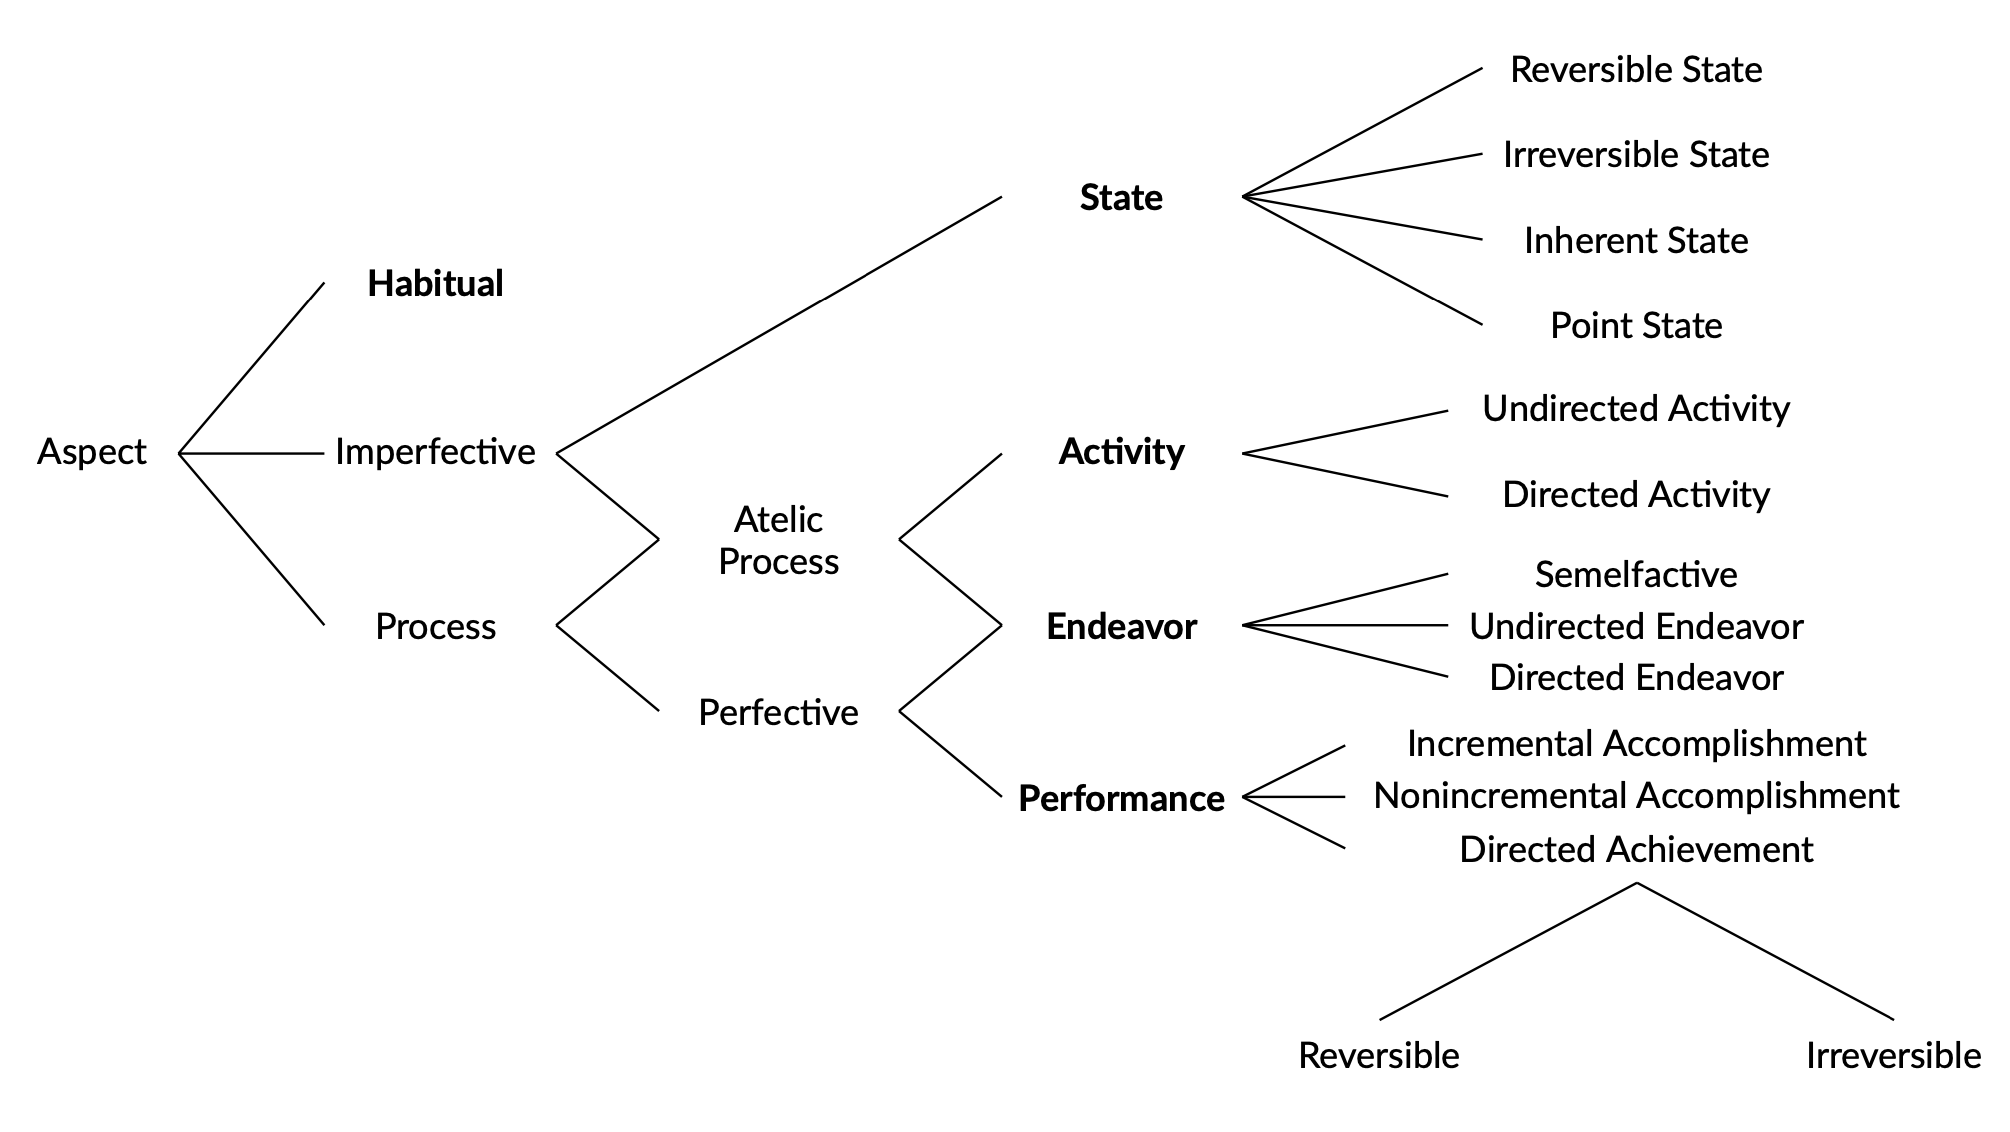
\includegraphics[width=\textwidth]{img/umr_aspct_tree.png}
    \caption{UMR aspect classification lattice \citep{umrslides2022}}
    \label{fig:umr_aspect_tree}
\end{figure}

How these relate to other aspectual classification schemata can be seen in table \ref{table:aspect_classes_comparison}.

Interesting to note is that these classes conflate the distinction made earlier between lexical and grammatical aspect, most clearly in the class "habitual", which is (in almost all cases) a paradigmatic example of an outer aspect, rather than one inherent in the verb event itself. Therefore, as can be seen in figure \ref{fig:umr_aspect_tree}, while classes which would usually be seen as grammatical aspect are to be found nearer the top of the tree (on the left), the leaves further down the tree are more examples of \emph{Aktionsarten}. That \citet{umr} make no mention of these different types of aspect is not necessarily surprising, given one of the main design goals of UMR is scalability, which entails learnability for annotators. As already mentioned, the theoretical distinction of inner and outer aspect is "very difficult to apply in practice" \citep{Dahl1985TenseAA}, hence a clear separation would often be difficult - and indeed not very fruitful - for annotators. Furthermore, this conflation of two phenomena can also be an advantage, since it shows the relationship between classes of each type (i.e. that \emph{irreversible states} are imperfective and \emph{directed achievements} perfective etc.), subsuming them all into \emph{one} semantic parameter space concerning aspect.

\begin{table}[]
    \begin{adjustbox}{width=\textwidth}
    \begin{tabular}{|l|l|l|l|l|l|l|}
    \hline
    \citet*{vendler57} &  \citet*{moens-steedman-1988-temporal}& \citet*{egg2005flexible} & \multicolumn{3}{l}{\citet*{annotAndAutoClassOfAspectCat}}  \vline & \citet{umr} \\ \hline \hline
\multirow{2}{*}{state}         & state                      & stative predicate     & \multicolumn{3}{l}{stative} \vline & \textbf{state} \\ \cline{2-7}
                               & (habitual state)           & (CHECK THIS)          & \multicolumn{3}{l}{-} \vline & \textbf{habitual} \\ \hline
activity                       & \multirow{2}{*}{process}   & process predicate     & \multirow{5}{*}{dynamic} & \multicolumn{2}{l}{unbounded} \vline & \textbf{activity} \\ \cline{1-1}\cline{3-3}\cline{5-7}
\multirow{2}{*}{accomplishment}&                            & intergressive predicate&      & \multirow{4}{*}{bounded} &  extended/no change & \textbf{endeavour} \\ \cline{2-3}\cline{6-7}
                               & culminated process         & change predicate      &       &  & extended/change & \textbf{performance}\\ \cline{1-3}\cline{6-7}
\multirow{2}{*}{achievement}   & point                      & intergressive predicate&      &  & punctual/no change & \textbf{endeavour} \\ \cline{2-3} \cline{6-7}
                               & culmination                & change predicate      &       &  & punctual/change & \textbf{performance} \\ \hline

    \end{tabular}
    \end{adjustbox}
    \caption{(Approximate) Comparison of aspectual classes. Adapted and extended from \citet*{annotAndAutoClassOfAspectCat}.}
    \label{table:aspect_classes_comparison}
\end{table}

\subsection*{Difficulties with aspect in UMR}
The UMR aspect system does come with some difficulties. Firstly, the classification scheme is notably different from those that came before it, since it is neither based on Vendler's classification, nor on typical binary aspect parameters, but rather seeks to create a typologically-informed aspect classification, taking into account explicit aspect encoding systems from a variety of languages. For example, the highest distinction made by \citet{comrie1976aspect} was between \textsc{perfective} and \textsc{imperfective}, while in UMR there are classes such as \textsc{endeavor} which can be both. The independence from the classic aspect parameters such as \textsc{telicity} or \textsc{durativity} also means the datasets annotated for one of these parameters cannot be easily used.

Secondly, UMR and its annotation guidelines are relatively new, hence sometimes unclear and are subject to change. This means that there are currently some minor inconsistencies between the annotated data available and the guidelines are sometimes unclear or problematic. I hope that as the project grows and expands to other languages, the annotation guidelines will be revised and refined and the inconsistencies fewer. At time of writing,\footnote{June 2024} the version 1.0 of the annotation guidelines has not yet been released.
\section{Research questions}
This section describes the research questions which the following study aims to answer.
\subsection*{RQ1: Can we train a system to identify aspect classes?}
The first question I aim to look at is whether we can train a system to automatically classify verbs in context as one of several aspect classes. This has been done before (see \ref{sect:previous_asp_class}), however this is the first time, to the best of my knowledge, that a \emph{large} language model\footnote{Defined as having > 1 million parameters, compared to BERT's 345 million.} has been used for this task. If this model works well, it will be possible to use it to look at some linguistic questions, such as whether particular prefixes in Slavic languages tend towards certain aspect classes, or carrying out a typological analysis of aspectual ambiguity (RQ3). 
\subsection*{RQ2: Can we automatically identify aspectually ambiguous verbs/sentences and which classes they tend towards?}
Once I have a model which can accurately predict verbal aspect in context, the next question will be the more complex task of predicting aspectual ambiguity. At this stage it is also an interesting question to examine how verb phrases are classified without context. This could shed some light on inherent aspectual readings of verb phrases and thus answer the question of whether there are some verb phrases which are perhaps "underspecified" in the model's latent space (see \ref{sect:coerc_or_under}).
\subsection*{RQ3: How does aspectual ambiguity compare across languages? Can we study the typology of aspectualisation?}
Finally, I will attempt to investigate and compare aspectual ambiguity across languages, looking at whether languages with more explicit marking for aspect have less aspect ambiguity than those expressing aspect more implicitly. I plan to answer this both by looking at the ambiguity classification of verbs in context and also of the top \emph{n} verbs in languages without context.
\section{Project outline}
\subsection*{Step 1: Fine-tune LLM for aspect classification}
In order to use language models to investigate aspect, it is necessary to first understand how much current language models know about aspectual phenomena. To this end, I will fine-tune a large language model on a small dataset (since no large datasets are available for the aspect classification scheme I choose, UMR \citep{umr}, or indeed in general for an aspect classification task), testing on a hold-out set. This step of fine-tuning a \emph{large} language model is necessary due to the scarcity of data available, which is not sufficient for fine-tuning a smaller model.
\subsection*{Step 2: Use fine-tuned LLM to annotate larger dataset}
The LLM fine-tuned in step 1 can then be used to annotate a larger dataset. Having a larger dataset allows a lot more possibilities for analysis than the dataset used for fine-tuning the larger model. For instance, this larger dataset can be used in a knowledge distillation (KD) process to train a smaller (possibly multilingual) model, which is useful for latent space analysis or comparison across languages. Though it must be noted that there is a danger of error propagation at this step.
\subsection*{Step 3: Compare aspectual systems cross-lingually}
Once we have training data of good enough quality, we can use this to train a multilingual model and use this to compare between languages. Here we can test the model in different contexts and use this to gain insights about the aspect systems of different languages, both in their own right and in comparison with one another, for example, to see if prevalence of aspectual ambiguity changes depending on how overtly a language marks for aspect, or if certain prefixes in a language mark a particular aspect class.

\subsection*{Step 4: Fine-tune LLM for aspect ambiguity detection}
In order to look at aspect ambiguity specifically, I will also fine-tune an LLM in a similar way to above to identify whether a verb in context has an ambiguous aspectual reading or not. However, since there does not yet exist a dataset annotated for aspectual ambiguity,\footnote{Recall that \citet{Friedrich2014AutomaticPO} only annotate ambiguity in the \textsc{dynamic/stative} parameter.} this part requires human annotation. I propose to solve this by requiring annotators to label sentence-verb pairs with any labels they see plausible. This makes it possible to have both a human class annotation and a derived ambiguity annotation for datapoints labelled with several labels. Neural networks are known for being overly confident in their predictions, and I will investigate whether low certainty of the smaller aspect \emph{classification} model (i.e. similar logit values across classes) correlates with the output of the model specially trained for ambiguity recognition.

\section{Use of LMs as sources of linguistic knowledge: Reversing the NLP pipeline}
One of the aims of this thesis is to highlight how language models can possibly be useful as sources of linguistic knowledge too. This idea is by no means new, and yet in the wider linguistics community outside computational linguistics, these tools seem to be little used.

Currently, the two main approaches used to develop and validate linguistic hypotheses are through corpora and through introspection, the former being championed by empiricists and the latter by the Chomskyan rationalist tradition \citep{corpus_textbook}. It is clear that corpora, including those used to train LLMs, can only contain a fraction of the famously infinite set of possible grammatical sentences in a language, and this has led Chomsky to decry corpus linguistics as seeking to model language \emph{performance} rather than \emph{competence} \citep{corpus_textbook}. Native speaker introspection, on the other hand, while able to judge the grammaticality of any sentence, is clearly highly subjective and biased. Language models, however, are productive and are able to generalise across their corpora to produce, with some sophistication, sentences not seen before in training, thus blurring the line between the traditional Chomskyan distinction between competence and performance.

While in the past, the NLP pipeline used to be made up of a host of linguistically informed steps (such as lemmatisation, dependency parsing and POS tagging), this changed with the advent of transformer models, which, some have argued, "rediscover" the classical NLP pipeline, albeit implicitly \citep{tenney2019bert}. Since these end-to-end models no longer require explicit linguistic encoding, one could argue that the importance of linguistic knowledge in NLP has dramatically decreased \citep{Church2021}, though it is undoubtedly true that linguistics is very useful for some areas of NLP which are currently less deep-learning inclined, such as low-resource NLP or meaning representation. Whether or not linguistics has a future in NLP, in this study I wish to look at the other direction of information flow and show that the benefits of collaboration between linguistics and NLP are not a one-way street.

\subsection*{When can (L)LMs \emph{not} help us?}
However, in light of the current hype surrounding deep learning it is important to highlight the limitations of such techniques and what language models \emph{cannot} do. 

It is well-known that training the LMs discussed in this paper requires a large amount of data and computing resources. While pre-trained models mean that LMs trained on relatively large amounts of data are now available for general use, for less well-resourced languages finding datasets of the necessary order of magnitude is a problem, and their performance suffers drastically. While this does not rule out the use of LMs on such languages (see \citep{kholodna2024llms}), it certainly limits the applicability and validity of some of the experiments described in this thesis to less well-resourced languages.

Furthermore, it must also be noted that LMs take on any biases present in the training data, meaning the language they approximate should be treated with caution. Examining these biases, as has often been done before, can, however, be an area of study in its own right and can produce valuable data for sociolinguistics. However, it must also be noted that it cannot be guaranteed that characteristics of a model's latent space can be transferred to a more general linguistic space, since human linguistic competence and LM competence differ in some aspects. Further research is therefore needed in this area.

Finally, since LMs are trained to minimize error on one variety of a language, they are less well-suited to study linguistic variation, whether geographical or temporal. This makes their use less suitable for languages without an accepted standard variant, such as Swiss German. In these cases, however, an approach using word embeddings with added dimensions such as \citet{hamilton-etal-2016-diachronic} could still be useful.

\clearpage
\chapter{Dataset Creation}\label{c.dataset}

RENAME THIS CHAPTER DATASET CREATION??????

\section{Dataset creation - should this go inside experiments?}
\label{sec:dataset_creation}
In order to carry out further computational analysis of the topic it is helpful to have an annotated dataset. Since no extensive datasets exist beyond for certain aspectual parameters such as telicity \citep{friedrich-gateva-2017-classification} or stativity \citep{Friedrich2014AutomaticPO}, I had to create my own \citep{friedrich-etal-2023-kind}. The traditional route of hand-annotating including has been a standard paradigm for many years however is highly time-intensive. Crowdsourcing is a more time- and cost-effective way of creating data, however has been shown to be of variable quality \citep{li2024comparative}, especially when the task requires more expert knowledge. Furthermore there are a range of biases which can affect data quality \citep{Beck2023}. The huge success of Large Language Models in recent years has prompted some to look at utilising them for dataset annotation either combined with human annotators \citep{goel2023llms} or on their own \citep{he2023annollm, llmsForPragAndDiscAnalysis, Gilardi_2023}, which is what I opted for.

\subsection{Dataset annotation with LLMs}
Large Language Models' use for annotation data has been demonstrated GIVE SOME EXAMPLES.  

\citet{törnberg2024best} formulated a set of best practices when using LLMs as text annotators, which I aim to be guided by. The paper provides guidelines for those wishing to use LLMs as text annotators, in the absence of labelled data. This situation differs from the "paradigmatic" one described in the paper by the fact that there already exist annotation guidelines and limited labelled data, hence the iterative systematic coding procedure described in the paper is not necessary. Nevertheless \citet{törnberg2024best} provides a well-needed framework for this relatively new approach. 

\subsubsection*{Choice of LM model}
There has been an explosion of LMs in recent years .....

While many previous studies looking at LLM capabilities choose to look at ChatGPT models due to their notoriety in recent years and general good performance. However, as \citet{törnberg2024best} notes, these models come with several issues: it is unknown what the training data for the model is, leading to problems with transparency, and ChatGPT models have been shown to evolve over time, meaning reproducability is hindered. For these reasons, and also in order to host the model locally for better control (rather than using an API), I chose to use a different model. Meta's Llama 2 model seemed to offer a good balance between the apparent current trade-off between performance and scientific good practice, performing comparatively well in previous studies \citep{yuan2023futureTimeLlama} + OTHER EXAMPLES

Due to hardware constraints, I had to use a technique to improve the efficiency of the model training process since the smallest Llama model is 7 billion parameters. In this case I chose to use PEFT (Parameter efficint fine-tuning) (ADD CITATION), which leverages the insight that LM fine-tuning usually only updates parameters at the end of the model. This made it possible to fine-tune the model without resorting to the huge amount of computing power usually necessary for fine-tuning LLMs.

I experimented both with the standard \textsf{Llama-2-7b} and \textsf{Llama-2-7b-chat} \citep{touvron2023llama}, however the latter ended up having difficulties responding in a formulaic way and rather added unnecessary or unrelated information, which is to be expected since it has been fine-tuned to fare well in a dialogue environment. This made it often difficult to extract the model's predicted label to use for evaluation. 

During the course of this study, Llama 3 was released to the public CITE LLAMA 3, promising to have better reasoning skills and be better at following instructions effectively, so I therefore tried and compared both models in comparable settings.

\subsubsection*{Training data}
As the only currently existing data containing UMR aspect classes, I used the example UMR dataset\footnote{ENTER LINK FOR WHERE TO FIND IT!!!!!!} provided by the creators of UMR. It contains HOW MANY sentences in 6 languages (Arapaho, Chinese, English, Kukama, Navajo and Sanapana) annotated according to the UMR schema. The texts come from WHERE 

In order to extract the verbs in the sentences I used Stanford NLP's Stanza POS tagger CITEEE, utilising the alignment given in the training data to find the corresponding node in the UMR graph and its aspect annotation. Table \ref*{umr_aspect_data} shows the class distribution of verbal events extracted from the dataset.
\begin{table}
    \centering
    \begin{tabular}{|c|c|c|c|}
        Class & No. examples in UMR data & No. examples in upsampling data & \textbf{Total} \\ \hline
        Performance & 124 & 1 & 125\\
        State & 55 & 0 & 55\\
        Activity & 36 & 2 & 38\\
        Endeavour & 17 & 14 & 31\\
        Habitual & 2 & 31 & 33\\ \hline
        \textbf{Total} & 234 & 48 & 282
    \end{tabular}
    \caption{Aspect classes of annotated verbal events in the UMR dataset.}
\end{table}
\label{umr_aspect_data}

Here it is clear that the \emph{habitual} class is underrepresented, corroborating the results of \citet{Dahl1985TenseAA}'s study concluding that habituals and related aspect classes have a low frequency in actual use, and hence I manually added some datapoints to improve the balance. The added sentences were either found in existing online datasets and simly labelled with a UMR aspect class by hand or they were both manually composed and then labelled.

\citet{törnberg2024best} points out that, since it is unknown exactly which training data was used to train many LMs, one should exercise caution when evaluating their performance on a test set, since the model may have seen the test data before during pre-training. In this case, while it is impossible to rule out that the UMR dataset was used for Llama 2 pretraining, it is highly unlikely that it has seen the data in this form (i.e. as a sentence, a verb from this sentence and a UMR aspect label for this verb), and since the model was pre-trained with a next-token prediction task, it is very improbable that it would have memorised the labels for the data it is being tested on in my experiments. Nevertheless this cannot be ruled out and must be kept in mind when analysing the results.

One interesting feature of the UMR \texttt{:aspect} parameter, is that it is used not only with verbs in the source sentence but also with nouns and adjectives (see for example \ref{nominal_event}).

\begin{figure}[t]
    (s1p / publication-91 \\
    \null\quad :ARG1 (s1l / landslide-01 \\
    \null\quad \quad:ARG3 (s1a / and \\
    \null\quad \quad\quad:op1 (s1d / die-01 \\
    \null\quad \quad\quad\quad:ARG1 (s1p3 / person :quant 200) \\
    \null\quad \quad\quad\quad:aspect state) \\
    \null\quad \quad\quad:op2 (s1f / fear-01 \\
    \null\quad \quad\quad\quad:ARG1 (s1m / miss-01 \\
    \null\quad \quad\quad\quad\quad:ARG1 (s1p2 / person :quant 1500) \\
    \null\quad \quad\quad\quad\quad:aspect state) \\
    \null\quad \quad\quad\quad:aspect state) \\
    \null\quad \quad\quad:aspect process) \\
    \null\quad :place (s1c / country :wiki "Philippines"  \\
    \null\quad \quad:name (s1n / name :op1 "Philippines"))))
    \caption{UMR graph of \emph{200 dead, 1,500 feared missing in Philippines landslide.}}
\end{figure}
\label{nominal_event}

Since Russian NLP tools are scarce, it would be difficult to perform event extraction, so, in order to keep the results comparable between both languages, I chose to just to focus on verbal events. In my analysis the \texttt{:aspect} parameter occurred with a verb in the source sentence $74.8\%$ of the time, meaning most of the data from the UMR dataset could be used.

\subsubsection*{Prompt engineering}
Prompt engineering is a new but important field in NLP, and studies have shown the importance of good prompts when dealing with LLMs \citep{kaddour2023challenges, hsieh2023automatic, sahoo2024systematic}. \citet{törnberg2024best} recommends an iterative prompt engineering process of 

The model was given the following instruction for each datapoint:
\begin{quotation}
    The annotation distinguishes five base level aspectual values—State, Habitual, Activity, Endeavor, and Performance. The State value corresponds to stative events: no change occurs during the event. It also includes predicate nominals (be a doctor), predicate locations (be in the forest), and thetic (presentational) possession (have a cat). The Habitual value is annotated on events that occur regularly in the past or present. The Activity value indicates an event has not necessarily ended and may be ongoing at Document Creation Time (DCT). Endeavor is used for processes that end without reaching completion (i.e., termination), whereas Performance is used for processes that reach a completed result state. 
\end{quotation}
followed by the following question:
\begin{quotation}
    Which class does "\emph{\{verb\}}" belong to in this sentence: state, habitual, activity, endeavor, or performance?"
\end{quotation}

\begin{table}
    \centering
    \begin{tabular}{|c|c|c|}\hline
        \textbf{Prompt type} & \textbf{Llama 2 7B} & \textbf{Llama 3 8B} \\ \hline
        No definitions & 0.198 & 0.479 \\ \hline
        Normal  & 0.748 & 0.769 \\\hline
        Long & 0.688 & 0.740  \\ \hline
    \end{tabular}
    \caption{F1 score on test set from fine-tuning Llama 2 7B and 3 8B on different types of prompt}
\end{table}

The results show that without an explanation of the classes, the model fails, achieving roughly random accuracy. WHICH EPOCH ARE THESE RESULTS FORMATINGG

Interestingly the results also show that the extended prompt (WHERE TO LINK THIS) also exhibited poorer performance. This could be due to the fact that it contained more redundant information which is 

\subsubsection*{Quantitative analysis of results}

\begin{table}
    \centering
    \begin{tabular}{|c|c|c|c|c|}\hline
        \textbf{Class} & \textbf{Precision} & \textbf{Recall} & \textbf{F1-Score} & \textbf{Support} \\ \hline
        Performance & 0.90 & 0.56 & 0.69 & 16\\ \hline
        State & 0.00 & 0.00 & 0.00 & 2\\\hline
        Activity & 0.88 & 0.58 & 0.70 & 12\\\hline
        Endeavour & 0.50 & 0.50 & 0.50 & 4\\\hline
        Habitual & 0.76 & 1.00 & 0.86 & 37\\ \hline \hline
        \textbf{Accuracy} &  &  & 0.77 & 71 \\ \hline
        \textbf{Macro Avg.} & 0.61  & 0.53 & 0.55 & 71 \\ \hline
        \textbf{Weighted Avg.} & 0.77  & 0.77 & 0.75 & 71 \\ \hline

    \end{tabular}
    \caption{Results on test set from fine-tuning Llama 2 on UMR aspect classes without upsampling. (UPDATE FORMATINGG!!!!!)}
\end{table}
\label{llama_results_no_upsampling}

\begin{table}
    \centering
    \begin{tabular}{|c|c|c|c|c|}\hline
        \textbf{Class} & \textbf{Precision} & \textbf{Recall} & \textbf{F1-Score} & \textbf{Support} \\ \hline
        Performance & 0.78 & 0.88 & 0.82 & 16\\ \hline
        State & 1.00 & 0.75 & 0.86 & 8\\\hline
        Activity & 1.00 & 0.56 & 0.71 & 9\\\hline
        Endeavour & 0.89 & 0.62 & 0.73 & 13\\\hline
        Habitual & 0.81 & 0.97 & 0.88 & 39\\ \hline \hline
        \textbf{Accuracy} &  &  & 0.84 & 85 \\ \hline
        \textbf{Macro Avg.} & 0.90  & 0.75 & 0.80 & 85 \\ \hline
        \textbf{Weighted Avg.} & 0.85  & 0.84 & 0.83 & 85 \\ \hline

    \end{tabular}
    \caption{Results on test set from fine-tuning Llama 2 on UMR aspect classes with upsampling. (UPDATE FORMATINGG!!!!!)}
\end{table}
\label{llama_results_upsampling}

The models seemed to learn the aspect classes relatively well, and it is clear that in general, manual upsampling improved results across the board, as is to be expected. However, the comparison of this result to the one on the model trained without upsampled data should be taken with a grain of salt, since the testing set also included some upsampled data (as there were not enough of some classes - mostly habituals - to make it a fair test), which are by design more prototypical and thus "easier" than the natural data. Nevertheless, this result taken as a standalone one shows that the model was capable of recognising occurrences of the five UMR aspect classes with relatively high accuracy.

\subsection{(Manual!!) Ambiguity annotation}
Since there are no existing datasets for aspectual ambiguity, I decided to annotate the training data I created for the Llama model. This means that I end up with a database of ambiguous sentences which can later be used for testing. This is a relatively hard task for annotation since it is rather open-ended (with $\sum_{i=1}^{5} \binom{5}{i}=31$ different possible annotations for a verb-sentence pair), and the interpretation of aspect is often rather a subjective process.

The annotation was done by an English native-speaker with a background in philosophy and myself. The annotators were given a detailed description of the UMR classes and asked to assign a class to each sentence-verb pair. If several readings were possible, the annotators were asked to write down all possibilities, indicating an aspectually ambiguous sentence. The annotators were also given the possibility to indicate when they were unsure on a particular sentence. See \ref{App:annguide} for the exact annotation guidelines.

For example, the following sentence-verb pair was annotated as belonging to \texttt{State} and \texttt{Activity} classes and hence has an ambiguous aspectual reading:

\begin{exe}
    \ex[] {The first footage from the devastated village showed a sea of mud covering what had been lush green valley farmland. \textbf{covering}}
\end{exe}
\label{ambigExampleSent}

\subsubsection{(Manual!!) Annotation results}

The results of the annotations can be seen in table \ref{table:annot_results}.

\begin{table}
    \begin{tabular}{|c|c|c|c|c|}\hline
        & \multicolumn{2}{|c|}{Annotator 1} & \multicolumn{2}{|c|}{Annotator 2} \\
         & Absolute freq. & Proportion & Absolute freq. & Proportion  \\ \hline
        Agreement with UMR\footnotemark & 202 & 0.706 & 202 & 0.706 \\ \hline
        Several labels (ambiguous) & 71 & 0.248 & 71 & 0.248 \\\hline
        Unsure & 28 & 0.098 & 28 & 0.098\\\hline
    \end{tabular}
    \footnotetext{This is defined as at least one of the classes labelled being the same as the class in the UMR dataset.}
    \caption{Analysis of annotated data. GET FOOTNOTE TO WORK HERE!!! AND UPDATE FOR ANNOTATOR 2}
\end{table}
\label{table:annot_results}

It was interesting to note that the majority of occurrences of the habitual class (30 out of 34 or 88\% AND WHAT FOR ANNOTATOR 2) were also annotated with other labels, empirically motivating the theory that habituality is located in a different level of aspectual distinction than the other classes. This is also reflected in the UMR aspect lattice (see figure \ref{fig:umr_aspect_tree}), where habituals are on the second highest level of the tree. 

Almost all (WHAT NUMBER) the sentence-verb pairs marked with several verb classes by annotator 1 were also marked as ambiguous by annotator 2, however only WHAT PERCENTAGE of those classified as ambiguous by the latter were seen as such by annotator 1. This causes a problem with 

(DIFFERENT SETUP NOW)This presents a problem in how to design the experiment set-up. Since we want to encourage the model to learn prototypical examples of aspect classes to make sure it is not overly confident on ambiguous datapoints, it would make sense to remove the datapoints labelled as having more than one class from training set. However, this would lead to the habitual class being almost non-existant in the dataset. One solution would be to leave them in labelled as habituals, but this would lead to WHAT WOULD IT LEAD TO

I therefore chose to keep datapoints which are 

\subsubsection{Consequences for aspectology}
Habitual on a different level

\subsection{Larger dataset}
In order to fine-tune the smaller model, a larger dataset is needed than the 209 sentences in the UMR example dataset. The only requirements for this larger dataset are that it is representative, clean and has enough exmaples to train the smaller model. It would also be an advantage if it is a sentence-aligned multilingual corpus, since this would make it possible to test the performance of a multilingual model in other languages where there are no labelled data from the Llama model. 

WHY DID WE TAKE OUT HABITUAL? AND NOT ITERATIVE??


\clearpage
\chapter{Experiments}\label{c.experiments}
\section{Dataset creation}
\label{sec:dataset_creation}
In order to carry out further computational analysis of the topic it is helpful to have an annotated dataset. Since no extensive datasets exist for UMR, I had to create my own. The traditional route of hand-annotating including has been a standard paradigm for many years however is highly time-intensive. Crowdsourcing is a more time- and cost-effective way of creating data, however has been shown to be of variable quality \citep{li2024comparative}, especially when the task requires more expert knowledge. Furthermore, there are a range of biases which can affect data quality \citep{Beck2023}. The huge success of LLMs in recent years has prompted some to look at utilising them for dataset annotation, either combined with human annotators \citep{goel2023llms} or on their own \citep{he2023annollm, llmsForPragAndDiscAnalysis, Gilardi_2023}.

\subsection{Dataset annotation with LLMs}
\citet{törnberg2024best} formulated a set of best practices when using LLMs as text annotators, which I aim to be guided by. The paper provides guidelines for those wishing to use LLMs as text annotators, in the absence of labelled data. However, this differs from my situation, where there already exist annotation guidelines and limited labelled data, hence the iterative systematic coding procedure described in the paper is not necessary. Nevertheless, \citet{törnberg2024best} provides a well-needed framework for this relatively new approach. 

\subsubsection*{Choice of LM model}
While many previous studies looking at LLM capabilities choose to look at ChatGPT models due to their notoriety in recent years and general good performance, these models come with several issues, as \citet{törnberg2024best} notes: it is unknown what the training data for the model is, leading to problems with transparency, and ChatGPT models have been shown to evolve over time, meaning reproducability is hindered. For these reasons, and also in order to host the model locally for better control (rather than using an API), I chose to use a different model. Meta's Llama 2 model \citep{touvron2023llama} seemed to offer a good balance between the apparent current trade-off between performance and scientific good practice, performing comparatively well in previous studies \citep{yuan2023futureTimeLlama} + OTHER EXAMPLES

Due to hardware constraints, I had to use a technique to improve the efficiency of the model training process since the smallest Llama model is 7 billion parameters. In this case I chose to use PEFT (Parameter efficint fine-tuning) \citep{peft}, which leverages the insight that LM fine-tuning usually only updates parameters at the end of the network. This made it possible to fine-tune the model without resorting to the huge amount of computing power usually necessary for fine-tuning LLMs.

I experimented both with the standard \textsf{Llama-2-7b} and \textsf{Llama-2-7b-chat}, however the latter ended up having difficulties responding in a formulaic way and rather added unnecessary or unrelated information, which is to be expected since it has been fine-tuned to fare well in a dialogue environment. This made it often difficult to extract the model's predicted label to use for evaluation. 

During the course of this study, Llama 3 was released to the public \citep{meta2024llama3}, promising to have better reasoning skills and be better at following instructions effectively, so I therefore tried and compared both models in comparable settings.

\subsubsection*{Training data}
As the only currently existing data containing UMR aspect classes, I used the example UMR dataset\footnote{The UMR dataset can be found \hyperlink{https://umr4nlp.github.io/web/data.html}{here}.} provided by the creators of UMR. It contains 2022 sentences in 6 languages (Arapaho, Chinese, English, Kukama, Navajo and Sanapana) annotated according to the UMR schema. The texts are a mix of news, oral 

In order to extract the verbs in the sentences I used Stanford NLP's Stanza POS tagger CITEEE, utilising the alignment given in the training data to find the corresponding node in the UMR graph and its aspect annotation. Table \ref*{umr_aspect_data} shows the class distribution of verbal events extracted from the dataset.
\begin{table}
    \centering
    \begin{tabular}{|c|c|c|c|}
        Class & No. examples in UMR data & No. examples in upsampling data & \textbf{Total} \\ \hline
        Performance & 124 & 1 & 125\\
        State & 55 & 0 & 55\\
        Activity & 36 & 2 & 38\\
        Endeavour & 17 & 14 & 31\\
        Habitual & 2 & 31 & 33\\ \hline
        \textbf{Total} & 234 & 48 & 282
    \end{tabular}
    \caption{Aspect classes of annotated verbal events in the UMR dataset.}
\end{table}
\label{umr_aspect_data}

Here it is clear that the \emph{habitual} class is underrepresented, corroborating the results of \citet{Dahl1985TenseAA}'s study concluding that habituals and related aspect classes have a low frequency in actual use, and hence I manually added some datapoints to improve the balance. The added sentences were either found in existing online datasets and simly labelled with a UMR aspect class by hand or they were both manually composed and then labelled.

\citet{törnberg2024best} points out that, since it is unknown exactly which training data was used to train many LMs, one should exercise caution when evaluating their performance on a test set, since the model may have seen the test data before during pre-training. In this case, while it is impossible to rule out that the UMR dataset was used for Llama 2 pretraining, it is highly unlikely that it has seen the data in this form (i.e. as a sentence, a verb from this sentence and a UMR aspect label for this verb), and since the model was pre-trained with a next-token prediction task, it is very improbable that it would have memorised the labels for the data it is being tested on in my experiments. Nevertheless this cannot be ruled out and must be kept in mind when analysing the results.

One interesting feature of the UMR \texttt{:aspect} parameter, is that it is used not only with verbs in the source sentence but also with nouns and adjectives (see for example \ref{nominal_event}).

\begin{figure}[t]
    (s1p / publication-91 \\
    \null\quad :ARG1 (s1l / landslide-01 \\
    \null\quad \quad:ARG3 (s1a / and \\
    \null\quad \quad\quad:op1 (s1d / die-01 \\
    \null\quad \quad\quad\quad:ARG1 (s1p3 / person :quant 200) \\
    \null\quad \quad\quad\quad:aspect state) \\
    \null\quad \quad\quad:op2 (s1f / fear-01 \\
    \null\quad \quad\quad\quad:ARG1 (s1m / miss-01 \\
    \null\quad \quad\quad\quad\quad:ARG1 (s1p2 / person :quant 1500) \\
    \null\quad \quad\quad\quad\quad:aspect state) \\
    \null\quad \quad\quad\quad:aspect state) \\
    \null\quad \quad\quad:aspect process) \\
    \null\quad :place (s1c / country :wiki "Philippines"  \\
    \null\quad \quad:name (s1n / name :op1 "Philippines"))))
    \caption{UMR graph of \emph{200 dead, 1,500 feared missing in Philippines landslide.}}
\end{figure}
\label{nominal_event}

Since Russian NLP tools are scarce, it would be difficult to perform event extraction, so, in order to keep the results comparable between both languages, I chose to just to focus on verbal events. In my analysis the \texttt{:aspect} parameter occurred with a verb in the source sentence $74.8\%$ of the time, meaning most of the data from the UMR dataset could be used.

\subsubsection*{Prompt engineering}
Prompt engineering is a new but important field in NLP, and studies have shown the importance of good prompts when dealing with LLMs \citep{kaddour2023challenges, hsieh2023automatic, sahoo2024systematic}. \citet{törnberg2024best} recommends an iterative prompt engineering process of 

The model was given the following instruction for each datapoint:
\begin{quotation}
    The annotation distinguishes five base level aspectual values—State, Habitual, Activity, Endeavor, and Performance. The State value corresponds to stative events: no change occurs during the event. It also includes predicate nominals (be a doctor), predicate locations (be in the forest), and thetic (presentational) possession (have a cat). The Habitual value is annotated on events that occur regularly in the past or present. The Activity value indicates an event has not necessarily ended and may be ongoing at Document Creation Time (DCT). Endeavor is used for processes that end without reaching completion (i.e., termination), whereas Performance is used for processes that reach a completed result state. 
\end{quotation}
followed by the following question:
\begin{quotation}
    Which class does "\emph{\{verb\}}" belong to in this sentence: state, habitual, activity, endeavor, or performance?"
\end{quotation}

\begin{table}
    \centering
    \begin{tabular}{|c|c|c|}\hline
        \textbf{Prompt type} & \textbf{Llama 2 7B} & \textbf{Llama 3 8B} \\ \hline
        No definitions & 0.198 & 0.479 \\ \hline
        Normal  & 0.748 & 0.769 \\\hline
        Long & 0.688 & 0.740  \\ \hline
    \end{tabular}
    \caption{F1 score on test set from fine-tuning Llama 2 7B and 3 8B on different types of prompt}
\end{table}

The results show that without an explanation of the classes, the model fails, achieving roughly random accuracy. WHICH EPOCH ARE THESE RESULTS FORMATINGG

Interestingly the results also show that the extended prompt (WHERE TO LINK THIS) also exhibited poorer performance. This could be due to the fact that it contained more redundant information which is 

\subsubsection*{Quantitative analysis of results}

\begin{table}
    \centering
    \begin{tabular}{|c|c|c|c|c|}\hline
        \textbf{Class} & \textbf{Precision} & \textbf{Recall} & \textbf{F1-Score} & \textbf{Support} \\ \hline
        Performance & 0.90 & 0.56 & 0.69 & 16\\ \hline
        State & 0.00 & 0.00 & 0.00 & 2\\\hline
        Activity & 0.88 & 0.58 & 0.70 & 12\\\hline
        Endeavour & 0.50 & 0.50 & 0.50 & 4\\\hline
        Habitual & 0.76 & 1.00 & 0.86 & 37\\ \hline \hline
        \textbf{Accuracy} &  &  & 0.77 & 71 \\ \hline
        \textbf{Macro Avg.} & 0.61  & 0.53 & 0.55 & 71 \\ \hline
        \textbf{Weighted Avg.} & 0.77  & 0.77 & 0.75 & 71 \\ \hline

    \end{tabular}
    \caption{Results on test set from fine-tuning Llama 2 on UMR aspect classes without upsampling. (UPDATE FORMATINGG!!!!!)}
\end{table}
\label{llama_results_no_upsampling}

\begin{table}
    \centering
    \begin{tabular}{|c|c|c|c|c|}\hline
        \textbf{Class} & \textbf{Precision} & \textbf{Recall} & \textbf{F1-Score} & \textbf{Support} \\ \hline
        Performance & 0.78 & 0.88 & 0.82 & 16\\ \hline
        State & 1.00 & 0.75 & 0.86 & 8\\\hline
        Activity & 1.00 & 0.56 & 0.71 & 9\\\hline
        Endeavour & 0.89 & 0.62 & 0.73 & 13\\\hline
        Habitual & 0.81 & 0.97 & 0.88 & 39\\ \hline \hline
        \textbf{Accuracy} &  &  & 0.84 & 85 \\ \hline
        \textbf{Macro Avg.} & 0.90  & 0.75 & 0.80 & 85 \\ \hline
        \textbf{Weighted Avg.} & 0.85  & 0.84 & 0.83 & 85 \\ \hline

    \end{tabular}
    \caption{Results on test set from fine-tuning Llama 2 on UMR aspect classes with upsampling. (UPDATE FORMATINGG!!!!!)}
\end{table}
\label{llama_results_upsampling}

The models seemed to learn the aspect classes relatively well, and it is clear that in general, manual upsampling improved results across the board, as is to be expected. However, the comparison of this result to the one on the model trained without upsampled data should be taken with a grain of salt, since the testing set also included some upsampled data (as there were not enough of some classes - mostly habituals - to make it a fair test), which are by design more prototypical and thus "easier" than the natural data. Nevertheless, this result taken as a standalone one shows that the model was capable of recognising occurrences of the five UMR aspect classes with relatively high accuracy.

\subsection{(Manual!!) Ambiguity annotation}
\label{sect:manual_amb_annotation}
Since there are no existing datasets for aspectual ambiguity, I decided to annotate the training data I created for the Llama model. This means that I end up with a database of ambiguous sentences which can later be used for testing. This is a relatively hard task for annotation since it is rather open-ended (with $\sum_{i=1}^{5} \binom{5}{i}=31$ different possible annotations for a verb-sentence pair), and the interpretation of aspect is often rather a subjective process.

The annotation was done by an English native-speaker with a background in philosophy and myself. The annotators were given a detailed description of the UMR classes and asked to assign a class to each sentence-verb pair. If several readings were possible, the annotators were asked to write down all possibilities, indicating an aspectually ambiguous sentence. The annotators were also given the possibility to indicate when they were unsure on a particular sentence. See \ref{App:annguide} for the exact annotation guidelines.

For example, the following sentence-verb pair was annotated as belonging to \texttt{State} and \texttt{Activity} classes and hence has an ambiguous aspectual reading:

\begin{exe}
    \ex[] {The first footage from the devastated village showed a sea of mud covering what had been lush green valley farmland. \textbf{covering}}
\end{exe}
\label{ambigExampleSent}

\subsubsection{(Manual!!) Annotation results}

The results of the annotations can be seen in table \ref{table:annot_results}.

\begin{table}
    \begin{tabular}{|c|c|c|c|c|}\hline
        & \multicolumn{2}{|c|}{Annotator 1} & \multicolumn{2}{|c|}{Annotator 2} \\
         & Absolute freq. & Proportion & Absolute freq. & Proportion  \\ \hline
        Agreement with UMR\footnotemark & 202 & 0.706 & 202 & 0.706 \\ \hline
        Several labels (ambiguous) & 71 & 0.248 & 71 & 0.248 \\\hline
        Unsure & 28 & 0.098 & 28 & 0.098\\\hline
    \end{tabular}
    \footnotetext{This is defined as at least one of the classes labelled being the same as the class in the UMR dataset.}
    \caption{Analysis of annotated data. GET FOOTNOTE TO WORK HERE!!! AND UPDATE FOR ANNOTATOR 2}
\end{table}
\label{table:annot_results}

It was interesting to note that the majority of occurrences of the habitual class (30 out of 34 or 88\% AND WHAT FOR ANNOTATOR 2) were also annotated with other labels, empirically motivating the theory that habituality is located in a different level of aspectual distinction than the other classes. This is also reflected in the UMR aspect lattice (see figure \ref{fig:umr_aspect_tree}), where habituals are on the second highest level of the tree. 

Almost all (WHAT NUMBER) the sentence-verb pairs marked with several verb classes by annotator 1 were also marked as ambiguous by annotator 2, however only WHAT PERCENTAGE of those classified as ambiguous by the latter were seen as such by annotator 1. This causes a problem with 

(DIFFERENT SETUP NOW)This presents a problem in how to design the experiment set-up. Since we want to encourage the model to learn prototypical examples of aspect classes to make sure it is not overly confident on ambiguous datapoints, it would make sense to remove the datapoints labelled as having more than one class from training set. However, this would lead to the habitual class being almost non-existant in the dataset. One solution would be to leave them in labelled as habituals, but this would lead to WHAT WOULD IT LEAD TO

I therefore chose to keep datapoints which are 

\subsubsection{Consequences for aspectology}
Habitual on a different level

\subsection{Larger dataset}
In order to fine-tune the smaller model, a larger dataset is needed than the 209 sentences in the UMR example dataset. The only requirements for this larger dataset are that it is representative, clean and has enough exmaples to train the smaller model. It would also be an advantage if it is a sentence-aligned multilingual corpus, since this would make it possible to test the performance of a multilingual model in other languages where there are no labelled data from the Llama model. 

WHY DID WE TAKE OUT HABITUAL? AND NOT ITERATIVE??


\section{Aspect classification}

\subsection{BERT fine-tuning}
Due to their size (and the subsequent large amount of data stored in the parameters), it is hard to carry out probing on LLMs, and, due the fact that they appeared recently, there has been less time to develop probing techniques, hence I decided to train a smaller model of the BERT \citep{devlin2019bert} family. These require more data to fine-tune than LLMs, and hence I used the fine-tuned Llama model to generate more training data in a technique known as knowledge distillation (KD). Knowledge distillation involves using a larger 'teacher' model to train a smaller 'student' model, often reaching the same or similar accuracy with a significantly smaller model. While not being able to probe the larger Llama model, smaller models are still an interesting artefact to consider and 

Furthermore, the complexity of larger LMs (especially those trained for generation rather than sequence classification (CHECK THIS!!!!)) means that their embedding space is noisier than smaller models that have been fine-tuned. This makes it harder to do the sort of probing described in later in this chapter.


\subsection{Aspect latent space}
Figure \ref{fig:fine-tuned_aspect_latent_space} provides a visualization of the \texttt{[CLS]} token embedding of verb-sentence pairs in the training set, together with their aspect label, from which several interesting observations can be made. For instance, it is interesting to note the positioning of \texttt{habitual} instances between \texttt{state} and \texttt{activity}, which accurately captures their semantics as somewhere between the more generic, non-episodic state and activities, denoting "an event [that] has not necessarily ended and may be ongoing at Document Creation Time (DCT)" \citep{umr}.

\begin{figure}
    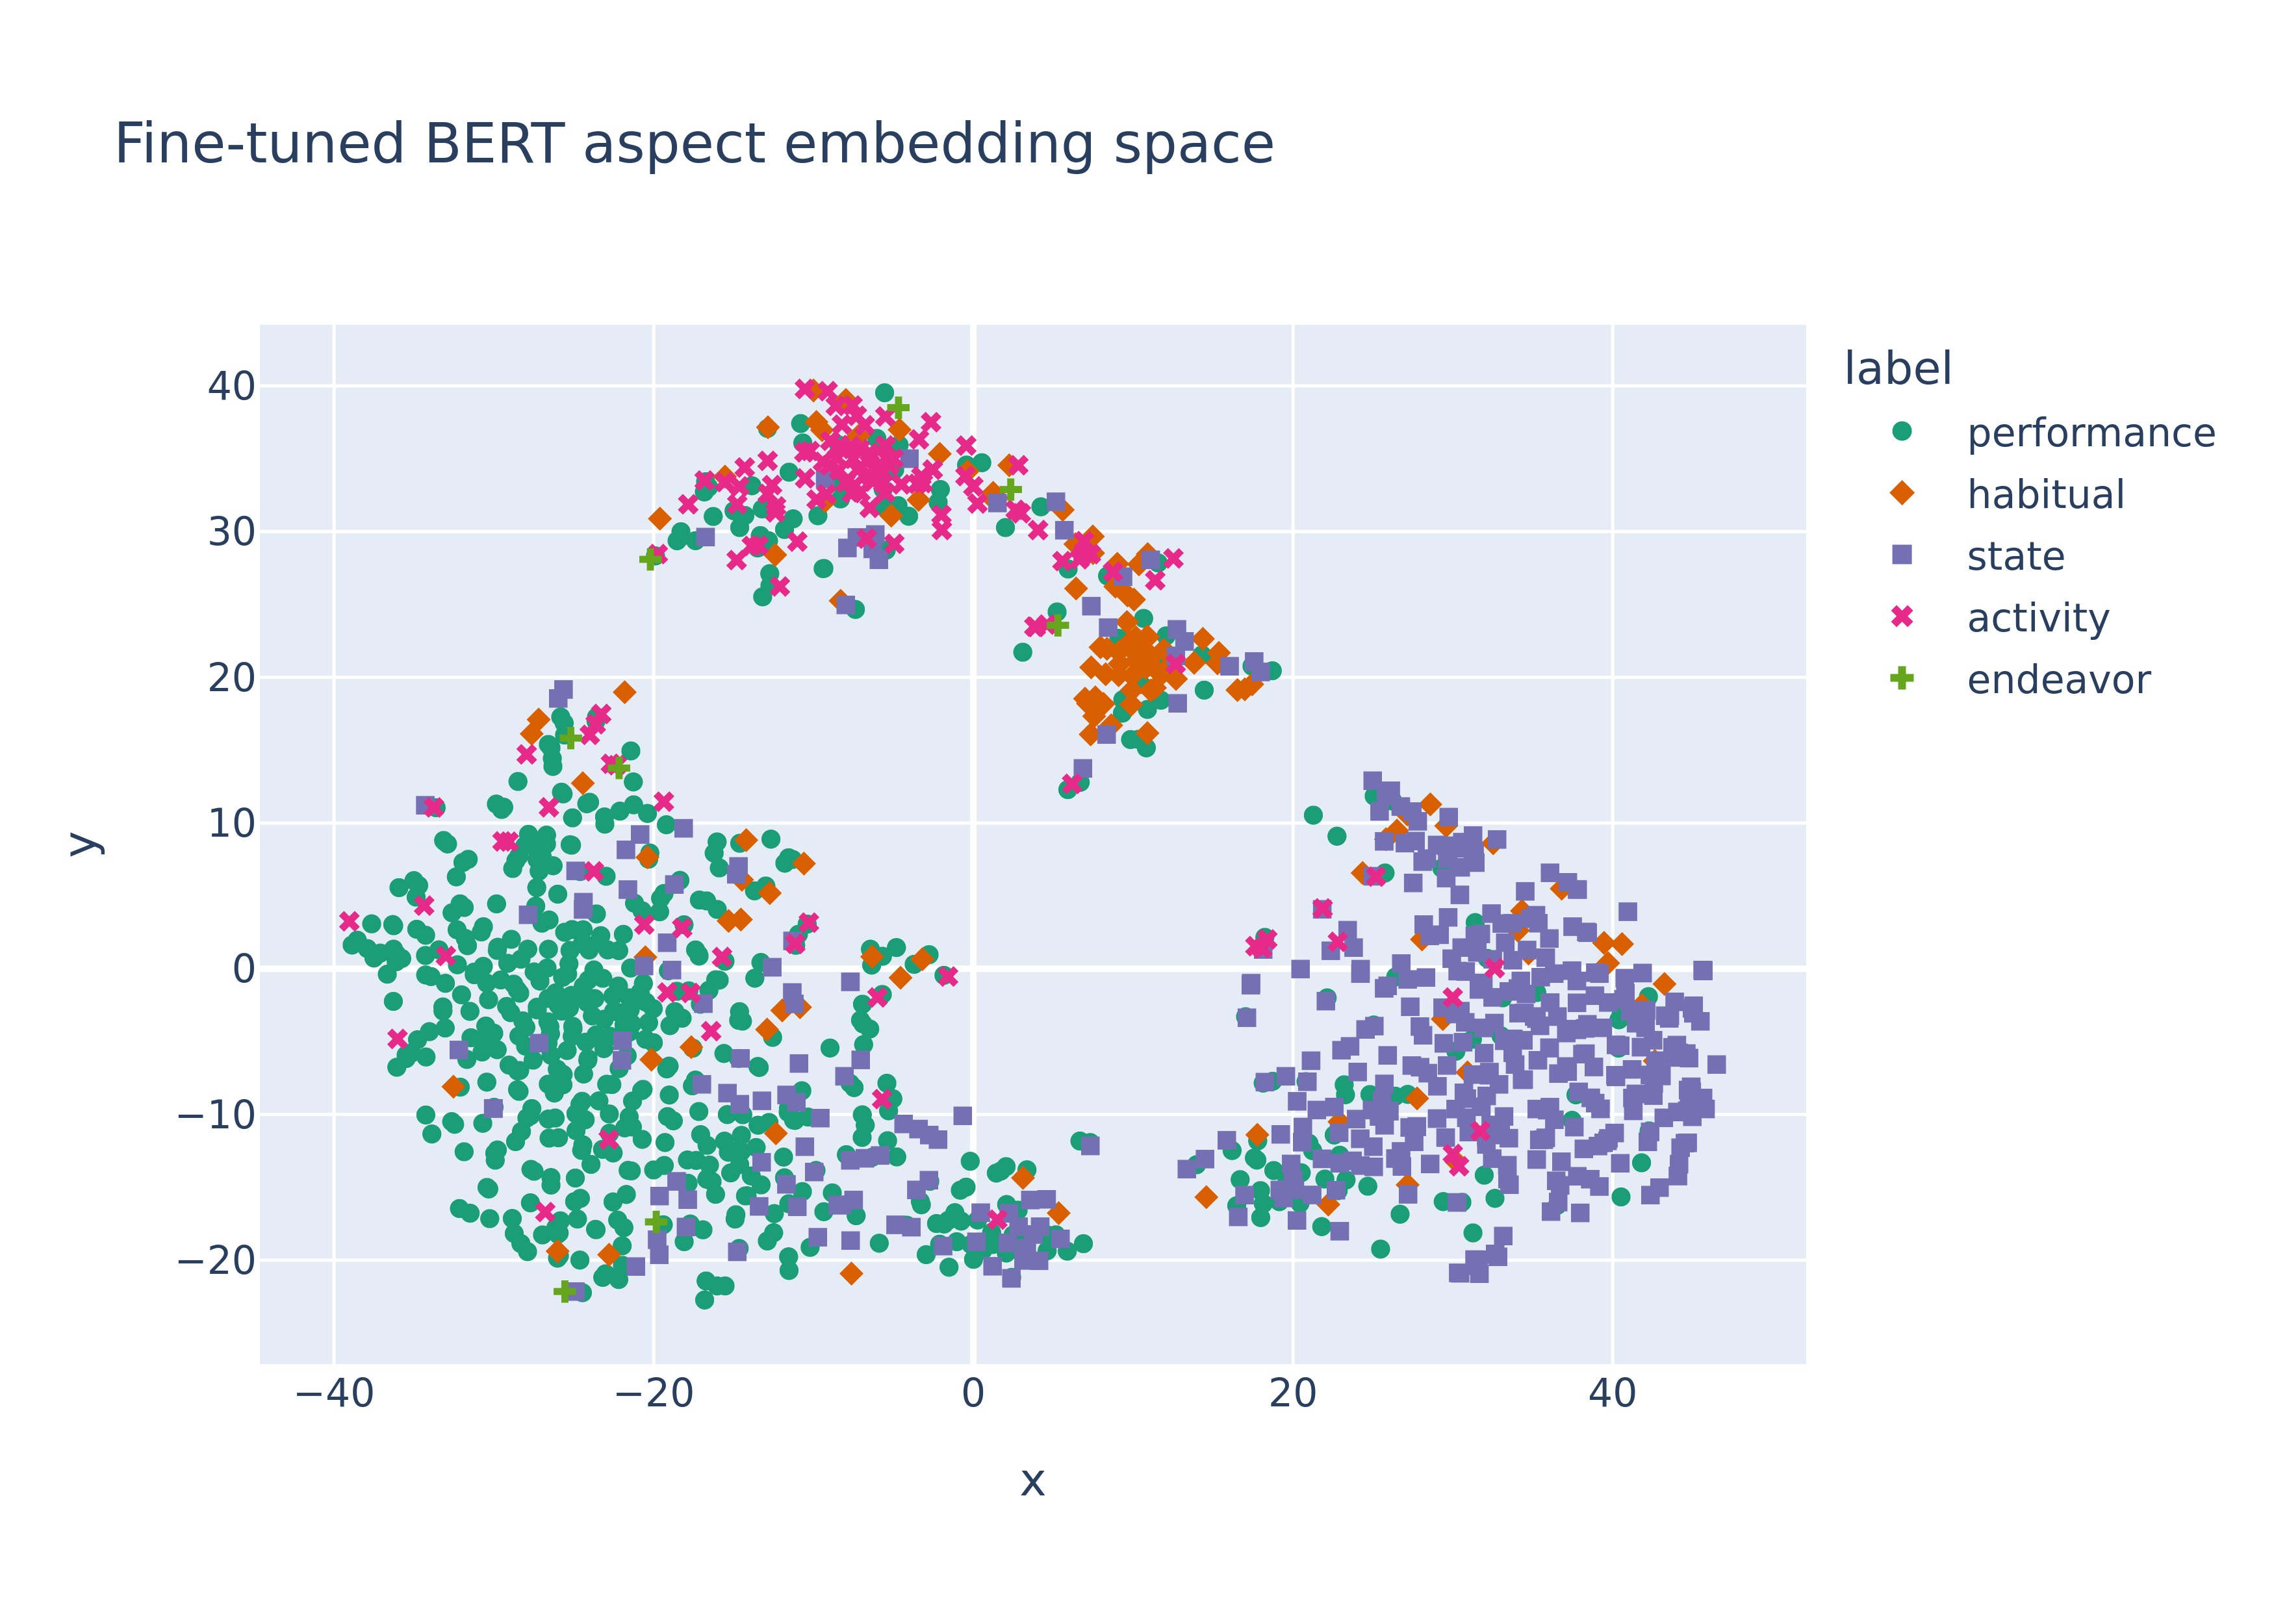
\includegraphics[width=\textwidth]{img/aspect_latent_space.jpeg}
    \caption{\texttt{[CLS]} embedding space of a BERT model fine-tuned on English verbs annotated for aspect in context, reduced to 2 dimensions by t-SNE.}
    \label{fig:fine-tuned_aspect_latent_space}
\end{figure}


\subsection{Multilingual BERT fine-tuning}
Since the LLM annotator Llama 3 can only be used in English, it is only possible to make training data in English. Luckily, however, there are multilingual models which can be trained with data using one language and then be used with languages other than that of the training data. I wanted to verify the performance of different models transferred to other languages and therefore needed a way of obtaining target labels for languages other than English.

I therefore trained a WHICH MODEL using WHICH DATASET annotated by the fine-tuned Llama 3 model and applied. The choice for this particular dataset was the availability of word-level alignments, a rarity in parallel corpora (IS THIS TRUE), meaning once a verb has been identified in the English sentence and given a particular aspect class, it is easy to find the corresponding verb in the other language. I only included sentences where the corresponding word in the other language is also a verb, since I wish to focus on verb phrases rather than general event classification.

In order to check the performance of this 

Get results in English and results in French

\begin{table}[h!]
    \centering
    \begin{tabular}{lcccc}
    \toprule
    \textbf{Model} & \multicolumn{2}{c}{\textbf{English}} & \multicolumn{2}{c}{\textbf{French}} \\
    \cmidrule(r){2-3} \cmidrule(r){4-5}
     & \textbf{F1 (best)} & \textbf{Acc} & \textbf{F1} & \textbf{Acc} \\
    \midrule
    \texttt{bert-base-multilingual-uncased} & 0.640 & 0.791 & 0.452 & 0.587 \\
    \texttt{bert-base-multilingual-cased}   & 0.647 & 0.790 & 0.450 & 0.572 \\
    \texttt{xlm-roberta-base}               & \textbf{0.665} & \textbf{0.813} & \textbf{0.522} & \textbf{0.651} \\
    \texttt{xlm-roberta-large}              & 0.647 & 0.797 & 0.447 & 0.629 \\
    \bottomrule
    \end{tabular}
    \caption{Model performance on English and French test sets after training on English training set.}
    \label{tab:performance}
    \end{table}

Hence, it is clear that the result is worse than in English, as is to be expected, however still significantly higher than chance.

\subsubsection{Russian aspect system}
As explained in \ref{sec:asp_in_slav_lang}


\subsubsection{Verb of motion clustering}
Unlike in English, almost all Russian imperfective verbs of motion have both a telic and an atelic counterpart. The former is used to describe a motion with a destination \ref{sent:telic_mv}, the latter for one without \ref{sent:atelic_mv}.

\begin{exe}
    \ex Ja \emph{šel} v školu. (I was walking to school.)
    \label{sent:telic_mv}
    \ex Ja \emph{chodil} po parku. (I was walking around the park.)
    \label{sent:atelic_mv}
\end{exe}

\begin{table}[h!]
    \centering
    \begin{tabular}{lllll}
    \textbf{Telic imperfective:} & Ja \emph{šel} v školu. &$\rightarrow $& \textsc{endeavour} & \checkmark\\
    \textbf{Telic perfective:} & Ja \emph{pošel} v školu. & $\rightarrow$ & \textsc{performance}  & \checkmark\\
    \textbf{Atelic imperfective:} & Ja \emph{guljal} po parku. & $\rightarrow$& \textsc{activity} & \checkmark\\
    \textbf{Atelic perfective:} & Ja \emph{poguljal} po parku. & $\rightarrow$& \textsc{activity} & ?\\
    \end{tabular}
    \caption{Model output of 3 example Russian sentences with motion verbs.}
    \label{tab:russian_mot_verb_outputs}
\end{table}

In UMR, events with no end goal are PROTOTYPISED? by activity, whereas telic events reaching completion are annotated with \texttt{performance}. We can verify that the model also makes this distinction HOW.

this empirically using the 

Using this we can 

\begin{table}[h!]
    \centering
    \begin{tabular}[t]{|l|c|c|r|l|}
        \hline
        \textbf{Verb} & & & \textbf{Entropy} & \textbf{PC} \\
        \hline
        schlappte &  &  & 0.00473 & performance\\
        schwebte &  &  & 0.00712 & activity\\
        trippelte &  &  & 0.00784 & activity\\
        schwankte &  &  & 0.00836 & activity\\
        schwamm &  &  & 0.00837 & activity\\
        pilgerte &  &  & 0.00856 & activity\\
        trabte &  &  & 0.00867 & activity\\
        strömten &  &  & 0.00877 & activity\\
        joggte &  &  & 0.00924 & activity\\
        flanierte &  &  & 0.00935 & activity\\
        tapste &  &  & 0.00943 & activity\\
        krabbelte &  &  & 0.00964 & activity\\
        watschelte &  &  & 0.0097 & performance\\
        latschte &  &  & 0.00996 & activity\\
        rutschte &  &  & 0.01028 & activity\\
        bummelte &  &  & 0.01128 & activity\\
        stromerten &  &  & 0.01148 & activity\\
        hüpfte &  &  & 0.01304 & activity\\
        purzelte &  &  & 0.01418 & activity\\
        schlurfte &  &  & 0.01443 & activity\\
        wanderte &  &  & 0.01623 & activity\\
        kullerte &  &  & 0.01686 & activity\\
        kroch &  &  & 0.01697 & activity\\
        hinkte &  &  & 0.01769 & activity\\
        schlich &  &  & 0.01799 & activity\\
        schweiften &  &  & 0.018 & activity\\
        streunten &  &  & 0.01959 & activity\\
        robbte &  &  & 0.01969 & activity\\
        wieselte &  &  & 0.0199 & activity\\
        glitt &  &  & 0.02027 & activity\\
        flatterte &  &  & 0.02123 & activity\\
        trampelte &  &  & 0.02399 & activity\\
        trieb &  &  & 0.0262 & activity\\
        hoppelte &  &  & 0.02664 & performance\\
        galoppierte &  &  & 0.02702 & activity\\
        wankte &  &  & 0.02801 & activity\\
        spazierte &  &  & 0.03137 & activity\\
        marschierte &  &  & 0.03802 & activity\\
        lief &  &  & 0.03966 & state\\
        reiste &  &  & 0.04599 & activity\\
        sprintete &  &  & 0.05367 & activity\\
    \end{tabular}
    \begin{tabular}[t]{|l|c|c|r|l|}
        \hline
        \textbf{Verb} & & & \textbf{Entropy} & \textbf{PC} \\
        \hline
        schlenderte &  &  & 0.05586 & activity\\
        tauchte &  &  & 0.05852 & activity\\
        hetzte &  &  & 0.06586 & activity\\
        ritt &  &  & 0.06784 & habitual\\
        taumelte &  &  & 0.07257 & activity\\
        trottete &  &  & 0.08606 & activity\\
        wandelte &  &  & 0.10565 & activity\\
        stolperte &  &  & 0.11249 & performance\\
        ruderte &  &  & 0.12711 & activity\\
        rannte &  &  & 0.13438 & activity\\
        tippelte &  &  & 0.1351 & performance\\
        torkelte &  &  & 0.13657 & activity\\
        tigerte &  &  & 0.16338 & activity\\
        skatete &  &  & 0.17054 & activity\\
        stieg &  &  & 0.17735 & endeavor\\
        humpelte &  &  & 0.18405 & activity\\
        radelte &  &  & 0.2051 & activity\\
        ging &  &  & 0.20655 & activity\\
        stapfte &  &  & 0.20949 & endeavor\\
        stapfte &  &  & 0.20949 & endeavor\\
        floh &  &  & 0.26129 & activity\\
        stolzierte &  &  & 0.33834 & activity\\
        huschte &  &  & 0.38448 & habitual\\
        fuhr &  &  & 0.39979 & performance\\
        raste &  &  & 0.40537 & activity\\
        kletterte &  &  & 0.44416 & habitual\\
        streifte &  &  & 0.49204 & activity\\
        hastete &  &  & 0.54362 & activity\\
        stürmte &  &  & 0.55842 & activity\\
        schritt &  &  & 0.5728 & performance\\
        eierte &  &  & 0.65506 & activity\\
        segelte &  &  & 0.67731 & activity\\
        sank &  &  & 0.74246 & performance\\
        sauste &  &  & 0.78209 & activity\\
        hopste &  &  & 0.78673 & endeavor\\
        flog &  &  & 0.84478 & activity\\
        flitzte &  &  & 0.85863 & activity\\
        rollte &  &  & 0.97166 & endeavor\\
        floss &  &  & 0.99165 & habitual\\
        sprang &  &  & 1.03842 & endeavor\\
        eilte &  &  & 1.27521 & activity\\
        \hline
    \end{tabular}
    \caption{CHANGE THIS}
\end{table}


\subsubsection{Prefix clustering}
An interesting application of this fine-tuned model is the 

ADD T-TEST FORMULA HERE

The probability of verbs with a prefix ($n=3489; \sigma = 0.3298; \mu = 0.1425$) being classified as the \textsc{state} class was lower than verbs without a prefix ($n=2473; \sigma = 0.4570; \mu = 0.3987$) by a statistically significant amount ($t = -25.1392; p < 1.3e-132$). This was also the case for the \textsc{activity} class, albeit by a much lesser degree ($t=-0.2841; p < 7.5e-2$). As can be seen in \ref{fig:fine-tuned_aspect_latent_space}, the opposite is also true for the \textsc{performance} class ($t=19.4150$), also with very high significance ($p<1.9e-081$). The differences between the \textsc{habitual} and \textsc{endeavour} classes was not significant.

This corroborates WHAT

\begin{figure}
    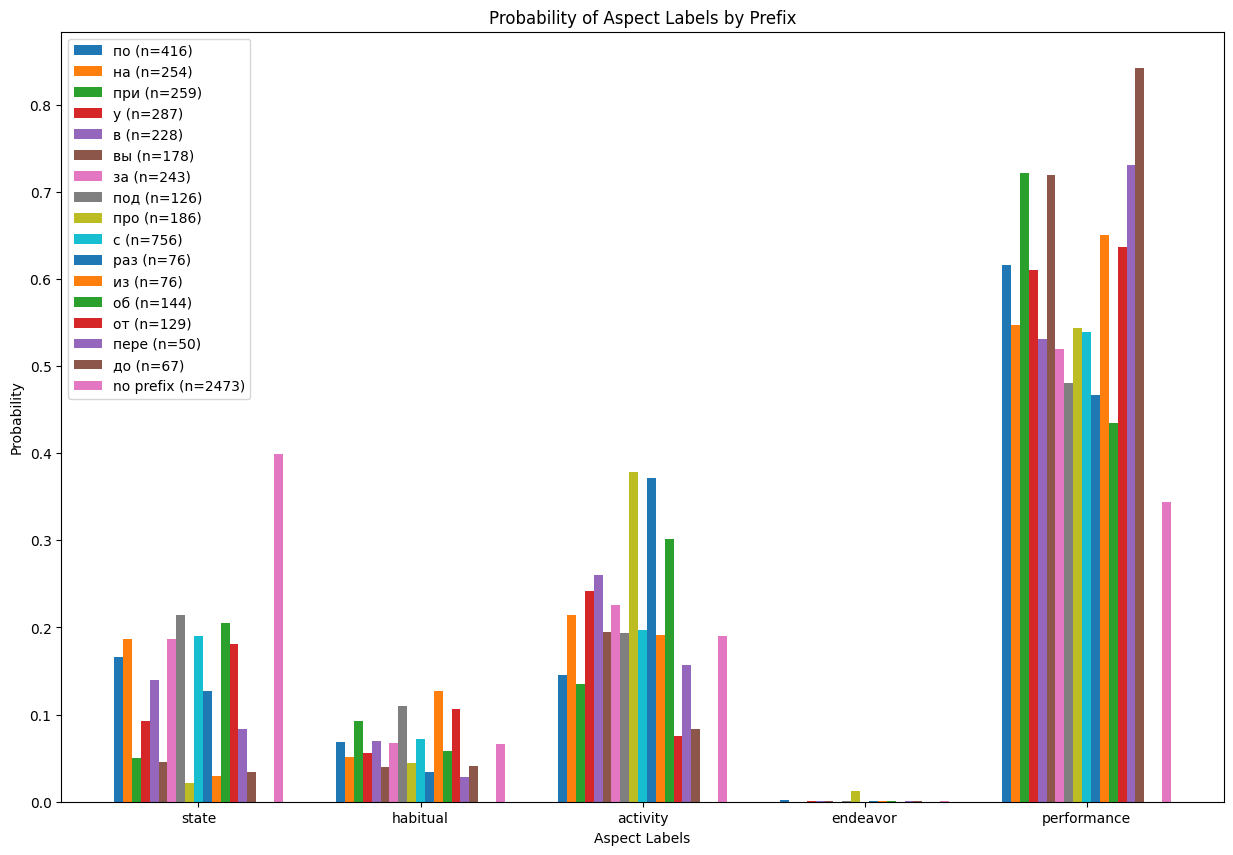
\includegraphics[width=\textwidth]{img/aspect_prediction_by_prefix.png}
    \caption{Look at this graph}
    \label{fig:fine-tuned_aspect_latent_space}
\end{figure}

Let's take the example of the prefixes \emph{pro-} (FIND OUT HOW TO ADD RUSSIAN HERE) and \emph{pere-}. While both meaning "through", they both emphasise different parts of the action. While \emph{pere-} simply implies that the "inceptive" and "terminal" limits of the domain being crossed have been traversed, \emph{pro-} puts emphasis on the action inside the domain and on the duration of this traversal \citep{0a0c5a60-a736-3226-b927-03ba8af4fd75}. This theoretical hypothesis is validated by the results here, with verbs beginning with \emph{pro-} exhibiting being classed significantly more often as \textsc{activity} ($t=3.2400; p<0.0014$).

both prefixes showing a significant difference in the 

\section{Aspectual ambiguity}
\subsection{Sentence-level ambiguity}
DOES ENTROPY CORRELATE WITH AMBIGUITY PREDICTION??
It is well known that LMs are often too confident of their predictions, even when wrong INSERT CITATION HERE

The first question that is interesting to ask (CHANGE DIESE FORMULIERUNG) is whether there is a correlation between the uncertainty of the aspect classification model and the output of the aspect ambiguity model, i.e. does a (supposed) ambiguous aspect reading of a sentence-verb pair correlate with uncertainty in the former's output. In order to quantify I take the concept of entropy and apply it to this case with the following formula:

$$H_{aspect} = - \sum_{i=1}^{\#AspClass}p(x_i)log(p(x_i))$$

In this way, higher uncertainty (i.e. a more balanced probability across all classes) leads to a higher $H_{aspect}$ value. It must be noted that this value is not comparable with models outputting a different number of classes (such as the traditional Vendlerian classification with 4), or indeed with different aspect classification systems (IS THIS TRUE??), however it serves the purpose for use to compare between languages (REWORD).

Using this value it is possible to calculate a correlation coefficient. The measure used was the point-biserial correlation coefficient, a metric mathematically equivalent to Pearson's correlation coefficient, however specialised for the case of one binary and one continuous variable. It is calculated thus:

$$r_{pb} = \frac{\overline{X}_1 - \overline{X}_0}{s} \sqrt{\frac{n_1 n_0}{n^2}}$$
where:
\begin{itemize}
    \item $\overline{X}_1$ is the mean of the continuous variable for the group where the binary variable is 1
    \item $\overline{X}_1$ is the mean of the continuous variable for the group where the binary variable is 0
    \item $s$ is the standard deviation of the continuous variable
    \item $n_1$ is the number of observations in the group where the binary variable is 1
    \item $n_0$ is the number of observations in the group where the binary variable is 0
    \item $n$ is the total number of observations
\end{itemize}

I found that the model entropy value had a \emph{medium}\footnote{According to Cohen's interpretation of Pearson's correlation \citep{cohen1988spa}} correlation of $\rho = 0.3465$ ($p < 0.0006$) with the upsampled ambiguity data derived from the human annotations. This is an encouraging result, especially the significance, however the correlation is not particularly high, and we should expect this value to be even lower for languages other than English, which sadly decreases the reliability of any conclusions taken from using the entropy value of this model. Furthermore, there was no correlation with the annotations of the fine-tuned LLM ($\rho = 0.0028; p < 0.85$), which is a disappointing result. 

Nevertheless, while this correlation with human is too small to lead to meaningful results on the level of individual datapoints, with a large enough sample size we can still use this to find general tendencies on the macro level, such as at language level.

\subsection{Verb-level ambiguity (TAKE OUT?)}

\subsection{Language-level ambiguity: Cross-linguistic comparison}

In order to compare between languages, it is first necessary to find a corpus available in the all the languages I wish to compare, if not parallel then with at least similar texts. To this end I decided to use TED2013 IS THIS TRUE???? corpus

Since I am comparing verbal ambiguity, I wished to 


\clearpage
\chapter{Discussion}\label{c.discussion}
Discussing the results.

It is clear that the model is far from perfect. 

\clearpage 
\chapter{Conclusion}\label{c.conclusion}
Verbal aspect is a prominent linguistic phenomenon.

In this thesis I have investigated the performance of current tools for aspect classification, using a classification schema taken from a larger meaning representation framework: UMR.

I exhibited some of the uses of this fine-tuned model for linguistics, such as Slavic prefix clustering with respect to aspect, and telicity detection in verbs of motion. Furthermore, I empirically validated the typological hypothesis that Slavic languages WHAT, using the language-level entropy

% Anhang
\clearpage
\appendix
\chapter{Appendix}
\section{Experiments with ChatGPT}
Over the last few years, Large Language Models (LLMs) such as GPT-3 \citep{gpt3} have achieved great amounts of success over a range of tasks in the NLP domain.

However, it has been shown that models such as ChatGPT struggle with mathematical and logical reasoning. 

\section{Temporal reasoning}

\section{Long LLM prompt}
\begin{quotation}
    \label{quote:long_prompt}
    Verbal aspect in language indicates how an action unfolds over time, emphasizing its internal structure, such as whether it is ongoing, completed, repeated, or momentary, distinct from tense which specifies when the action occurs relative to a reference point. The annotation distinguishes five base level aspectual values. The State value corresponds to stative events: no change occurs during the event. The Habitual value is annotated on events that occur regularly. The Activity value indicates an event with no inherent goal that has not necessarily ended and may be ongoing. Endeavor is used for processes which have an inherent end goal but which end without reaching completion (i.e., termination), whereas Performance is used for processes that reach a completed result state. Which class does "\emph{\{verb\}}" belong to in this sentence: state, habitual, activity, endeavor or performance?
\end{quotation}

\section{Annotation guidelines}
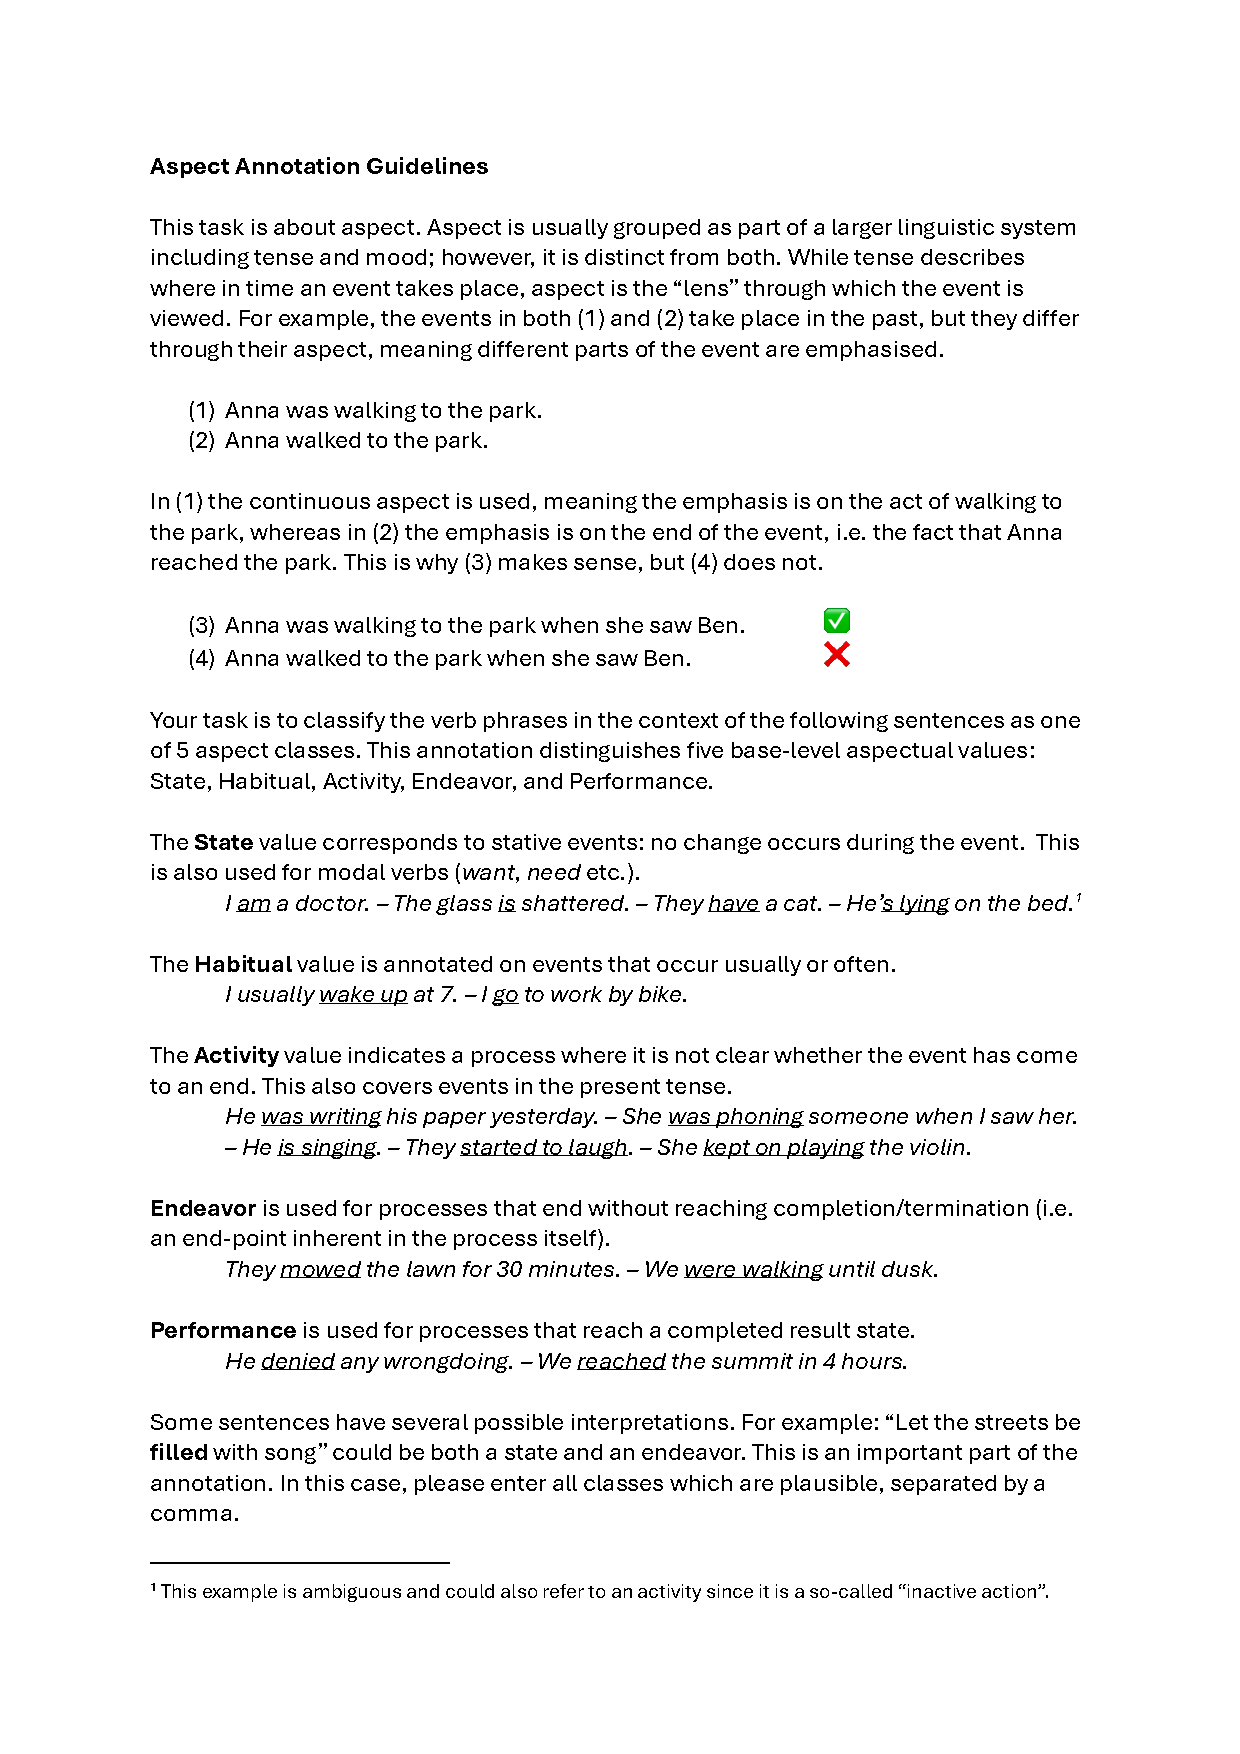
\includepdf[pages={-}]{img/ann_guide.pdf}
\label{App:annguide}

\section{Language-level entropy}
\label{App:lang_level_entropy_TED}
\begin{table}[ht]
    \centering
    \caption{Language-level Entropy on TED2013 dataset}
    \begin{tabular}{lcc}
        \toprule
        \textbf{Language} & \textbf{Mean Entropy} & \textbf{Variance} \\
        \midrule
        Chinese & $0.24579$ & $0.33647$ \\ \hline
        English & $0.32071$ & $0.19312$ \\
        German & $0.35085$ & $0.42130$ \\
        Dutch & $0.36985$ & $0.41680$ \\ \hline
        Italian & $0.36227$ & $0.42906$ \\
        Romanian & $0.33647$ & $0.40408$ \\
        Spanish & $0.36194$ & $0.43184$ \\
        Portuguese & $0.41209$ & $0.43718$ \\ \hline
        Polish & $0.31180$ & $0.41160$ \\
        Slovene & $0.29825$ & $0.38113$ \\
        Russian & $0.28984$ & $0.38741$ \\
        \bottomrule
    \end{tabular}
\end{table}

\begin{table}[ht]
    \centering
    \caption{Language-level Entropy on TED2020 dataset}
    \begin{tabular}{lcc}
        \toprule
        \textbf{Language} & \textbf{Mean Entropy} & \textbf{Variance} \\
        \midrule
        Arabic & $0.28453$ & $0.38861$ \\ \hline
        Vietnamese & $0.49336$ & $0.46466$ \\ \hline
        Chinese & $0.27207$ & $0.34002$ \\ \hline
        Danish & $0.43019$ & $0.42449$ \\
        Dutch & $0.36016$ & $0.41209$ \\
        English & $0.31668$ & $0.19319$ \\
        German & $0.34829$ & $0.42011$ \\
        Icelandic & $0.39461$ & $0.43853$ \\
        Norwegian Bokmål & $0.46367$ & $0.46847$ \\
        Norwegian Nynorsk & $0.42910$ & $0.46448$ \\
        Swedish & $0.42756$ & $0.46448$ \\ \hline
        Catalan & $0.45707$ & $0.48769$ \\
        French & $0.41091$ & $0.44966$ \\
        Italian & $0.36121$ & $0.42817$ \\
        Portuguese & $0.41012$ & $0.43479$ \\
        Romanian & $0.33490$ & $0.40521$ \\
        Spanish & $0.31668$ & $0.43953$ \\ \hline
        Estonian & $0.31668$ & $0.43953$ \\
        Finnish & $0.29564$ & $0.36784$ \\
        Hungarian & $0.32440$ & $0.39755$ \\ \hline
        Greek & $0.26212$ & $0.36320$ \\ \hline
        Latvian & $0.28655$ & $0.36055$ \\
        Lithuanian & $0.34829$ & $0.42011$ \\ \hline
        Belorussian & $0.28453$ & $0.38861$ \\
        Bulgarian & $0.28453$ & $0.38861$ \\
        Croatian & $0.27519$ & $0.37766$ \\
        Czech & $0.27519$ & $0.37766$ \\
        Polish & $0.30852$ & $0.40623$ \\
        Russian & $0.28529$ & $0.38692$ \\
        Slovakian & $0.28453$ & $0.38861$ \\
        Slovene & $0.28453$ & $0.38861$ \\
        Ukrainian & $0.24490$ & $0.35603$ \\
        \bottomrule
    \end{tabular}
\end{table}

\clearpage
%\bibliographystyle{natbib}
\bibliography{references}

\end{document}
